\documentclass[12pt,a4paper]{article}
\usepackage[utf8]{inputenc}
\usepackage[spanish]{babel}
\usepackage{amsmath}
\usepackage{amsfonts}
\usepackage{amssymb}
\usepackage{graphicx}
\usepackage[left=2cm,right=2cm,top=2cm,bottom=2cm]{geometry}

\usepackage{enumitem}
\usepackage{algorithm}
\usepackage{algorithmic}
\usepackage[hidelinks]{hyperref}

\usepackage{subcaption}
\usepackage{pgfplots}

% Para la tabla
\usepackage{multirow}
\usepackage[normalem]{ulem}
\useunder{\uline}{\ul}{}


\usepackage{listings}
\lstset{
	basicstyle=\ttfamily,
	columns=fullflexible,
	frame=single,
	breaklines=true,
	postbreak=\mbox{\textcolor{red}{$\hookrightarrow$}\space},
}


\author{Ignacio Aguilera Martos}
\title{Trabajo Integrador \\ Introducción a la Ciencia de Datos}
\date{22 de Diciembre de 2019}

\setlength{\parindent}{0cm}
\setlength{\parskip}{10px}


\begin{document}
	\maketitle

	\tableofcontents

	\newpage
	
\section{Análisis Exploratorio de los Datos}

En esta primera sección vamos a hacer una exploración de los datos intentando extraer algunas conclusiones de los mismos y poder conocer más en profundidad la información que nos arrojan las variables. Esta sección va a estar dividida en dos subsecciones, una para el conjunto de regresión y otra para el conjunto de clasificación.

\subsection{Conjunto de Regresión}

El conjunto de datos del que dispongo para realizar regresión es el conjunto ``treasury''. Vamos a analizar el conjunto de datos.

En primer lugar el conjunto de datos dispone de  16 variables numéricas y 1049 observaciones como podemos observar con el siguiente código.

\begin{figure}[H]
	\centering
	\begin{subfigure}{0.47\textwidth}
		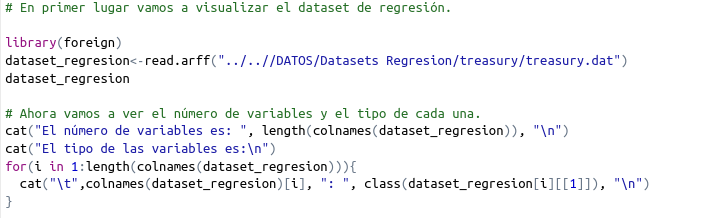
\includegraphics[scale=0.35]{./Imagenes/EDA/Regresion/codigo_variables_tipos.png}
	\end{subfigure}
	\begin{subfigure}{0.47\textwidth}
		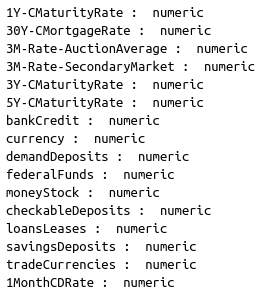
\includegraphics[scale=0.4]{./Imagenes/EDA/Regresion/variables_tipos.png}
	\end{subfigure}
	\caption{Tipos de las variables y código para obtenerlos}
\end{figure}

Como podemos ver el conjunto dispone de 16 variables de las cuales todas son numéricas. Esto es lógico pues el conjunto está destinado para el problema de regresión y además nos facilita el trabajo. 

Para poder seguir analizando el conjunto vamos a hacer un estudio pormenorizado de las variables del mismo en función a una serie de estadísticos básicos.

Estos estadísticos que voy a emplear son: media, mediana, moda, desviación típica, mínimo, máximo, curtosis y asimetría.

En este conjunto podemos dividir las variables en dos grupos. El primero de ellos corresponde a las variables de entrada que son las que nos van a permitir obtener resultados sobre la salida y el segundo grupo es la propia salida esperada del sistema.

Vamos a empezar a analizar en primer lugar la salida.

\subsubsection{Estudio de los estadísticos}

\subsubsection*{Salida}
La variable de salida es la que tiene por nombre 1MonthCDRate. Los estadísticos que nos arroja esta variable son los siguientes:

\begin{figure}[H]
	\centering
	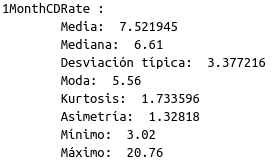
\includegraphics[scale=0.7]{./Imagenes/EDA/Regresion/estadisticos_1MonthCDRate.png}
	\caption{Estadísticos de la variable de salida.}
\end{figure}

Podemos observar que la  media de la salida es aproximadamente de $7.5$ y su desviación típica de $3.3$, esto nos indica que la mayoría de los datos (el 95\% en caso de estar ante una distribución normal) van a estar dentro del intervalo $[0.9,14,1]$. Aún así podemos ver mediante el mínimo y el máximo que los datos se van a mover en el intervalo $[3.02, 20.76]$. Esto parece que nos va a indicar que deberíamos de tener una cola más pesada a la izquierda de la distribución y una cola más alargada a la derecha de la misma. Este hecho viene corroborado también por la mediana. Vemos que es $6.61$ (menor que la media) con lo que nos está diciendo que el 50\% de los datos van a estar en el intervalo $[3.02, 6.61]$ y por tanto proporcionalmente esta cola será más pesada.

Otra forma que tenemos de comprobar lo que hemos dicho es mediante el coeficiente de asimetría. Al ser positivo nos está indicando que la distribución es asimétrica a la derecha, cuestión que ya sabemos y hemos razonado.

La curtosis nos está dando una indicación de cómo de puntiaguda o achatada es la distribución. En este caso el coeficiente es positivo, por lo que la distribución será más puntiaguda. Esto nos está indicando que vamos a tener una mayor concentración de datos entorno a la media.

\subsubsection*{Variable 1: 1Y-CMaturityRate}

Los estadísticos que nos arroja esta variable son:

\begin{figure}[H]
	\centering
	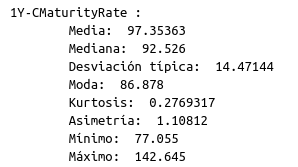
\includegraphics[scale=0.7]{./Imagenes/EDA/Regresion/estadisticos_1Y_CMaturityRate.png}
	\caption{Estadísticos de la variable 1 1Y\_CMaturityRate}
\end{figure}

En primer lugar podemos observar que la media es de $97.35363$ y la mediana es ligeramente inferior. Esto nos vuelve a indicar que vamos a tener una cola más corta a la izquierda y una más larga a la derecha, es decir, vamos a tener más valores a la derecha de la distribución. Podemos corroborar este hecho también comprobando el mínimo y el máximo. Como podemos ver el máximo está mucho más alejado de la media que el mínimo por lo que podemos intuir que la distribución va a ser más alargada por ese lado.

De igual forma si miramos el coeficiente de asimetría vemos que es positivo lo que nos está indicando la asimetría de la cola derecha.

La curtosis es positiva pero no muy lejana del cero, por lo que tendrá la forma de una normal pero un poco más puntiaguda.

\subsubsection*{Variable 2: 30Y-CMortgageRate}

Los estadísticos que nos arroja esta variable son:

\begin{figure}[H]
	\centering
	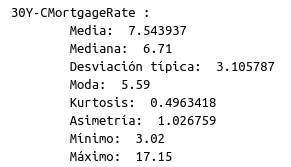
\includegraphics[scale=0.7]{./Imagenes/EDA/Regresion/estadisticos_30Y_CMortgageRate.png}
	\caption{Estadísticos de la variable 2 30Y\_CMortgageRate}
\end{figure}

Podemos ver que la media es $7.543937$ y la mediana $6.71$ lo que de nuevo nos hace sospechar que la cola derecha es más alargada. Esto lo podemos ver (y podemos decir ya que la cola va a ser bastante alargada) con el máximo y el mínimo. Sabemos que el 95\% de los datos debería de estar en el intervalo $[ media-2*stdv, media+2*stdv ]$ pero la realidad es que observamos que la cola derecha es más larga. Asimismo vemos que la moda es aún menor que la mediana con lo que corroboramos que la cola izquierda es más pesada y la derecha más alargada.

El coeficiente de asimetría nos termina de corroborar lo que estamos infiriendo pues al ser positivo nos indica una asimetría en la cola derecha.

En cuanto a la curtosis podemos ver que es más puntiaguda que una normal.

\subsubsection*{Variable 3: 3M-Rate-AuctionAverage}

Los estadísticos que nos arroja esta variable son:

\begin{figure}[H]
	\centering
	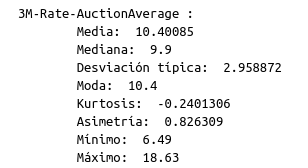
\includegraphics[scale=0.7]{./Imagenes/EDA/Regresion/estadisticos_3M_Rate_AuctionAverage.png}
	\caption{Estadísticos de la variable 3 3M\_Rate\_AuctionAverage}
\end{figure}

Esta variable tiene como media $10.40085$ y mediana $9.9$. En esta variable no vemos una diferencia tan grande por lo que a priori podemos pensar que no es muy asimétrica. La desviación típica es de $2.958872$ por lo que (en caso de que fuese una normal) el 95\% de los datos se van a encontrar en el intervalo $[4.483106, 16.318594]$. Vemos que el mínimo es $6.49$ con lo que podemos entender que la cola izquierda es más corta mientras que el máximo es $18.63$ con lo que la cola derecha va a ser algo más alargada.

Si observamos los coeficiente de asimetría y curtosis podemos ver que el coeficiente de asimetría es positivo lo que nos indica que la distribución es asimétrica a la derecha y la curtosis es ligeramente negativa con lo que podemos decir que la distribución será algo más achatada que una distribución normal.

\subsubsection*{Variable 4: 3M-Rate-SecondaryMarket}

Los estadísticos que nos arroja esta variable son:

\begin{figure}[H]
	\centering
	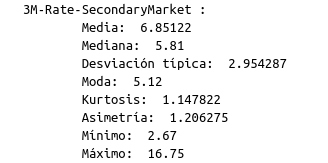
\includegraphics[scale=0.7]{./Imagenes/EDA/Regresion/estadisticos_3M_Rate_SecondaryMarket.png}
	\caption{Estadísticos de la variable 4 3M\_Rate\_SecondaryMarket}
\end{figure}

Podemos observar que el comportamiento de esta variable es el mismo que las anteriores y que va a tener una cola a la derecha más alargada. Esto es comprobable por todas las razones expuestas en las secciones anteriores.

\subsubsection*{Variable 5: 3Y-CMaturityRate}

Los estadísticos que nos arroja esta variable son:

\begin{figure}[H]
	\centering
	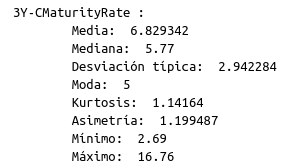
\includegraphics[scale=0.7]{./Imagenes/EDA/Regresion/estadisticos_3Y_CMaturityRate.png}
	\caption{Estadísticos de la variable 5 3Y\_CMaturityRate}
\end{figure}

De igual forma los estadísticos de esta variable nos están arrojando la misma información que para el resto de variables con una cola derecha muy alargada. Podemos corroborar esta información por lo mismo que hemos dicho antes (mediana, media, máximo y minino) además de coeficiente de asimetría que al ser positivo nos indica que es asimétrica a la derecha.

Por otro lado, al igual que en los casos previos, la curtosis nos indica que la distribución es más puntiaguda o apuntada que una distribución normal.

\subsubsection*{Variable 6: 5Y-CMaturityRate}

Los estadísticos que nos arroja esta variable son:

\begin{figure}[H]
	\centering
	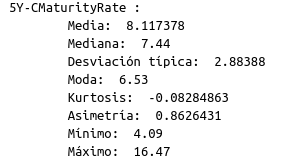
\includegraphics[scale=0.7]{./Imagenes/EDA/Regresion/estadisticos_5Y_CMaturityRate.png}
	\caption{Estadísticos de la variable 6 5Y\_CMaturityRate}
\end{figure}

En esta variable observamos también una cola derecha más alargada pero podemos observar que aquí no es una cola tan alargada como en los casos anteriores. 

Si comprobamos la media y la mediana observamos que la mediana es menor que la media por lo que ya nos está apuntando a la asimetría pero si vemos la desviación típica y calculamos el intervalo en el que deberían estar el 95\% de los datos ($[2.349618, 13,885138]$) podemos percibir que la cola izquierda es más corta (pues el mínimo es $4.09$) y la cola derecha más alargada pues el máximo llega hasta $16.47$.

Podemos decir que la asimetría derecha se manifiesta pero con menor intensidad como podemos percibir por el coeficiente de asimetría, pues aunque es positivo, es menor que en otros casos.

En cuanto a la curtosis podemos ver que es ligeramente negativa pero muy cercana al cero por lo que podemos decir que la distribución esta ligerísimamente achatada con respecto a una normal aunque visualmente probablemente no pudiéramos distinguirlo.

\subsubsection*{Variable 7: bankCredit}

Los estadísticos que nos arroja esta variable son:

\begin{figure}[H]
	\centering
	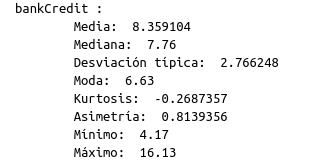
\includegraphics[scale=0.7]{./Imagenes/EDA/Regresion/estadisticos_bankCredit.png}
	\caption{Estadísticos de la variable 7 bankCredit}
\end{figure}

En este caso podemos ver que la mediana es más pequeña que la media por lo que podemos pensar de nuevo en que esta variable tiene una cola derecha más alargada. Si calculamos el intervalo en el que deberían de estar el 95\% de los datos ($[2.826608,13.8916]$) podemos apreciar esa tendencia a una cola derecha más pesada. 

Aún así, si comprobamos el coeficiente de asimetría, podemos ver que se manifiesta la asimetría derecha pero de forma ligera como en la variable anterior pues el coeficiente no es tan grande como en otras variables que ya hemos analizado. 

En cuanto a la curtosis tenemos una curtosis negativa lo que nos indica que la distribución está algo más achatada que su correspondiente distribución normal.

\subsubsection*{Variable 8: currency}

Los estadísticos que nos arroja esta variable son:

\begin{figure}[H]
	\centering
	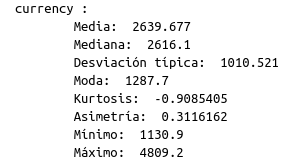
\includegraphics[scale=0.7]{./Imagenes/EDA/Regresion/estadisticos_currency.png}
	\caption{Estadísticos de la variable 8 currency}
\end{figure}

En este caso la mediana también es algo más pequeña que la media, pero si comprobamos el rango de valores de la variable ($[1130.9, 4809.2,]$) observamos que la diferencia no es tan significativa por lo que no podemos decir tan rápido que tenemos una cola derecha más alargada. Como vemos la desviación típica es de $1010.521$ por lo que el intervalo que debe contener el 95\% de los datos es $[618.635,4660,719]$. 

Con esta información podemos apuntar que debe existir una ligera asimetría en la cola derecha porque el mínimo es mayor que el mínimo que nos da el intervalo del 95\% de los datos y el máximo es algo mayor que el máximo del intervalo del 95\%.

Para contrastar esta información tenemos el coeficiente de asimetría que, al ser positivo, nos dice que la distribución presenta asimetría derecha pero podemos ver que es mucho más pequeño que en el resto de variables con lo que la asimetría no es tan pronunciada.

En cuanto a la curtosis podemos ver que es negativa por lo que la distribución es más achatada que una distribución normal.

\subsubsection*{Variable 9: demandDeposits}

Los estadísticos que nos arroja esta variable son:

\begin{figure}[H]
	\centering
	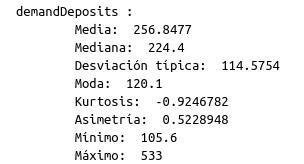
\includegraphics[scale=0.7]{./Imagenes/EDA/Regresion/estadisticos_demandDeposits.png}
	\caption{Estadísticos de la variable 9 demandDeposits}
\end{figure}

Como podemos observar tenemos que la mediana es menor que la media. Volvemos a tener una situación que nos lleva a pensar que tenemos una cola derecha más alargada que la izquierda.

Si calculamos el intervalo en el que debe estar el 95\% de los datos ($[27.6969,485.9985]$) podemos observar que el máximo es algo más grande que el máximo de dicho intervalo e igualmente ocurre con el mínimo con lo que tenemos un desplazamiento de los datos hacia la derecha.

El hecho viene refrendado por el coeficiente de asimetría que al ser positivo nos indica dicha asimetría derecha.

En cuanto a la curtosis al tener una curtosis negativa estamos ante una distribución más achatada que en el caso de una normal.

\subsubsection*{Variable 10: federalFunds}

Los estadísticos que nos arroja esta variable son:

\begin{figure}[H]
	\centering
	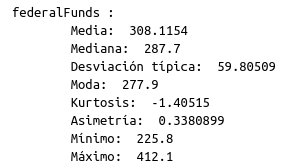
\includegraphics[scale=0.7]{./Imagenes/EDA/Regresion/estadisticos_federalFunds.png}
	\caption{Estadísticos de la variable 10 federalFunds}
\end{figure}

Podemos observar en esta variable el mismo comportamiento que venimos destacando del resto. Tenemos que la mediana es más pequeña que la media lo que nos indica que la cola derecha de la distribución debe ser algo más alargada.

El intervalo en el que el 95\% de los datos debe caer es $[188.50522, 427.72558]$. Podemos ver que el máximo de este intervalo es ligeramente más grande que el máximo y el mínimo es ligeramente más grande que el del intervalo del 95\% por lo que podemos decir que si existe una asimetría derecha esta no es muy pronunciada.

Podemos contrastar lo que estamos afirmando por el coeficiente de asimetría que es ligeramente positivo, por lo que se confirma lo que estamos razonando de que tenemos una ligera asimetría derecha.

En cuanto a la curtosis tenemos que es negativa y grande por lo que será muy achatada con respecto a una normal de mismos parámetros.

\subsubsection*{Variable 11: moneyStock}

Los estadísticos que nos arroja esta variable son:

\begin{figure}[H]
	\centering
	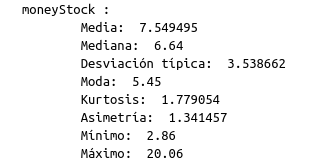
\includegraphics[scale=0.7]{./Imagenes/EDA/Regresion/estadisticos_moneyStock.png}
	\caption{Estadísticos de la variable 11 moneyStock}
\end{figure}

Podemos repetir exactamente el mismo razonamiento que hemos hecho anteriormente para argumentar la asimetría derecha, pero en este caso al comprobar el coeficiente de asimetría podemos ver que es mucho más pronunciada.

En cuanto a la curtosis tenemos el comportamiento opuesto al de la variable anterior teniendo que la distribución es significativamente más puntiaguda o apuntada que su normal de mismos parámetros.

\subsubsection*{Variable 12: moneyStock}

Los estadísticos que nos arroja esta variable son:

\begin{figure}[H]
	\centering
	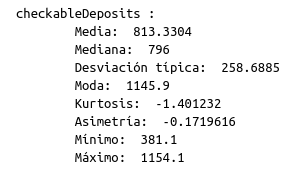
\includegraphics[scale=0.7]{./Imagenes/EDA/Regresion/estadisticos_checkableDeposits.png}
	\caption{Estadísticos de la variable 12 checkableDeposits}
\end{figure}

Este es el primer ejemplo en el que podemos ver como la cola más alargada no va a ser la cola derecha sino la izquierda. En este caso, al igual que los anteriores, podemos ver que la mediana es menor que la media (aunque no mucho proporcionalmente al rango de valores que se toman). Esto podría indicarnos que la cola derecha continúa siendo algo más alargada que la izquierda, pero en este caso podemos apreciar que la moda (el valor más frecuente) es significativamente más grande que la media, por lo que no podemos intuir un comportamiento a priori. Tenemos información contradictoria, una parte nos dice que debemos tener la cola derecha más alargada y la otra nos está diciendo que la izquierda es la que debería ser más alargada.

Para poder estudiar esta situación compleja recurrimos al coeficiente de asimetría. Como podemos ver en este caso es negativo pero ligeramente. Tal y como podíamos pensar la situación está razonablemente equilibrada aunque mostrando una ligera asimetría izquierda.

En cuanto a la curtosis tenemos que es negativa y grande, por lo que estamos ante una distribución mucho más achatada que una distribución normal de mismos parámetros.

\subsubsection*{Variable 13: savingsDeposits}

Los estadísticos que nos arroja esta variable son:

\begin{figure}[H]
	\centering
	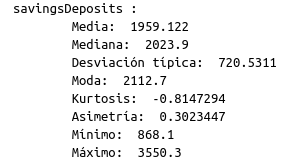
\includegraphics[scale=0.7]{./Imagenes/EDA/Regresion/estadisticos_savingsDeposits.png}
	\caption{Estadísticos de la variable 13 savingsDeposits}
\end{figure}

El caso de esta variable es singular también. Podemos ver que la mediana es mayor que la media, la moda también por lo que podríamos pensar que la cola más alargada es la izquierda. 

Por contra si miramos el intervalo minino y máximo podemos ver que lo más probable es que se extienda más la cola derecha pues el máximo es más grande proporcionalmente a la media que el mínimo. 

Para contrastar la información miramos el coeficiente de asimetría y observamos que, aunque es pequeño, es positivo. Esto nos indica que la distribución es asimétrica derecha.

Si analizamos la curtosis podemos ver que es negativa lo que nos indica que la distribución es más achatada que una normal de mismos parámetros.

\subsubsection*{Variable 14: tradeCurrencies}

Los estadísticos que nos arroja esta variable son:

\begin{figure}[H]
	\centering
	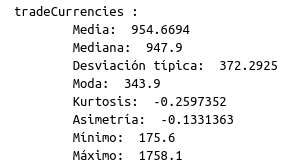
\includegraphics[scale=0.7]{./Imagenes/EDA/Regresion/estadisticos_tradeCurrencies.png}
	\caption{Estadísticos de la variable 14 tradeCurrencies}
\end{figure}

En cuanto a esta variable podemos ver que la media es mayor (ligeramente) que la mediana y la moda es mucho menor que la media. Por contra tenemos que el mínimo es más significativo que el máximo en cuanto al intervalo de valores se refiere. En ese caso a priori no podemos decir nada.

Si miramos el coeficiente de asimetría podemos contrastar esta información pues es muy cercano a cero y en este caso ligeramente negativo por lo que si podemos decir algo es que es ligeramente asimétrica la distribución a la izquierda.

La curtosis es ligeramente negativa por lo que podemos decir que es un poco más achatada que su normal asociada.



Cabe decir tras todo este estudio de estadísticos de las variables que podríamos hacer transformaciones que modifiquen nuestras variables para que cumplan una distribución normal. Por ejemplo es sabido que si tenemos distribuciones con asimetría derecha podemos solucionarlo en la mayoría de casos con una transformación logarítmica. Esto puede esperar hasta que probemos los modelos y comprobemos si es necesario.

\subsubsection{Estudio de la correlación de las variables}

En esta sección vamos a estudiar la correlación entre variables que no son de salida y de dichas variables con la de salida para intentar ver cuales van a ser las más relevantes para nuestro estudio o si hay alguna variable que podamos quitar.

En primer lugar vamos a hacer un estudio de la correlación entre las variables. Nuestro objetivo va a ser obtener aquellas que tienen alta correlación con otras variables, es decir, obtener aquellas variables que son explicadas por otras pues estas las podremos quitar.

Por supuesto todo este estudio habrá que contrastarlo sobre los resultados de la regresión, pero podemos hacer hipótesis previas al ajuste de los modelos.

El código que voy a emplear para el estudio es el siguiente:

\begin{figure}[H]
	\centering
	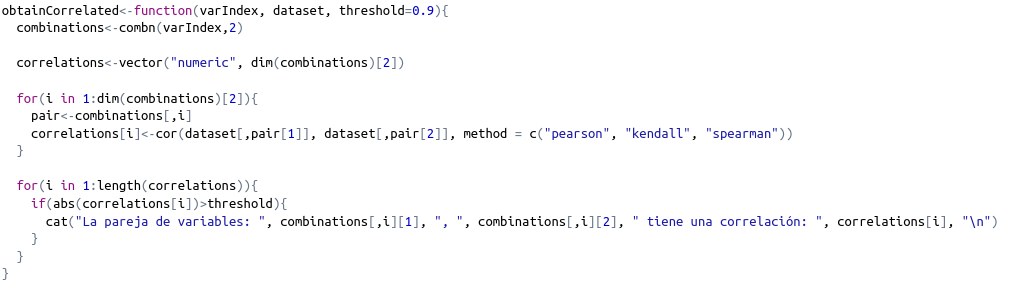
\includegraphics[scale=0.51]{./Imagenes/EDA/Regresion/correlacion_entre_variables_codigo.png}
	\caption{Código para el estudio de la correlación entre variables.}
\end{figure}

Para poder eliminar una variable de forma que estemos seguros de que no quitamos información debemos exigir que la correlación entre variables sea alta. En este caso como se puede ver en el código solamente vamos a mostrar las parejas de variables que presenten una correlación alta, en concreto que en valor absoluto sea mayor a $0.9$.

Vamos a ver las parejas de variables que cumplen esta condición.

\begin{figure}[H]
	\centering
	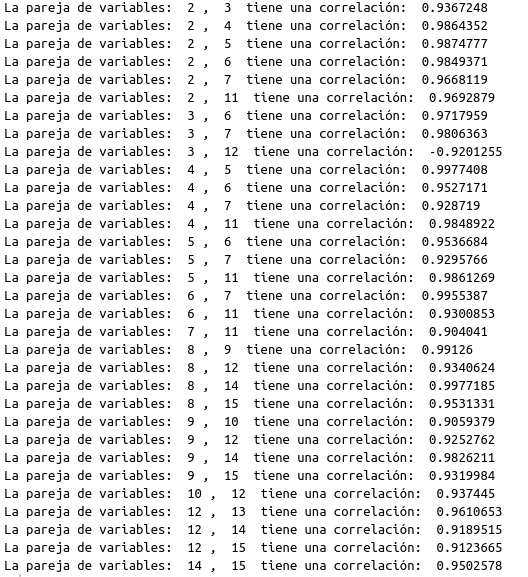
\includegraphics[scale=0.6]{./Imagenes/EDA/Regresion/correlacion_entre_variables1.png}
	\caption{Primer filtrado de la correlación entre variables}
\end{figure}

Podemos observar claramente que la variable 2 tiene una correlación muy alta con otras variables, por lo que podemos eliminarla al ser explicada por las variables 3,4,5,6,7 y 11.

\begin{figure}[H]
	\centering
	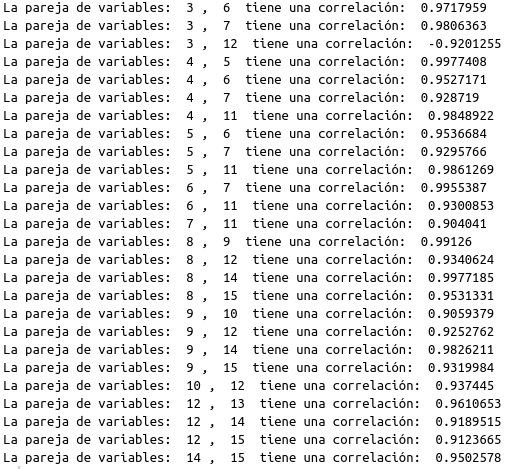
\includegraphics[scale=0.6]{./Imagenes/EDA/Regresion/correlacion_entre_variables2.png}
	\caption{Correlación entre variables después de eliminar la segunda.}
\end{figure}

Podemos ver a su vez que la variable 9 tiene una correlación muy alta con las variables 10, 12, 14 y 15 por lo que podemos eliminarla.

\begin{figure}[H]
	\centering
	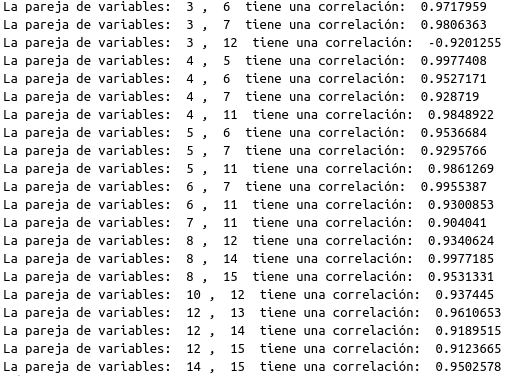
\includegraphics[scale=0.6]{./Imagenes/EDA/Regresion/correlacion_entre_variables3.png}
	\caption{Correlación entre variables después de eliminar la segunda y la novena.}
\end{figure}

La variable 4 podemos ver que tiene alta correlación con las variables 5,6,7 y 11 por lo que podemos quitarla también.

\begin{figure}[H]
	\centering
	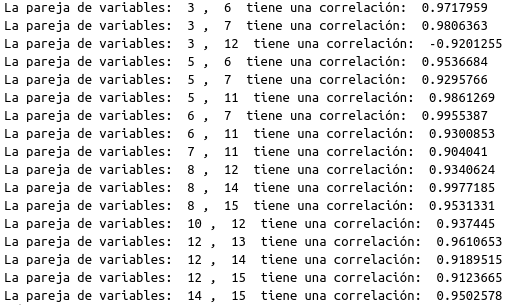
\includegraphics[scale=0.6]{./Imagenes/EDA/Regresion/correlacion_entre_variables4.png}
	\caption{Correlación entre variables después de eliminar la segunda, la novena y la cuarta.}
\end{figure}

La tercera variable sigue manteniendo una alta correlación con las variables 6,7 y 12, por lo que podemos eliminarla.

\begin{figure}[H]
	\centering
	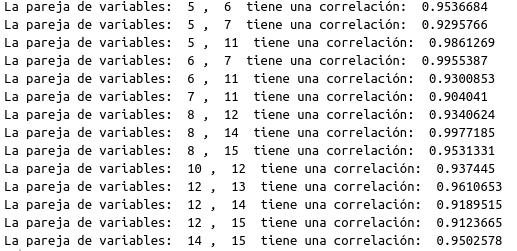
\includegraphics[scale=0.6]{./Imagenes/EDA/Regresion/correlacion_entre_variables5.png}
	\caption{Correlación entre variables después de eliminar la segunda, la novena, la cuarta y la tercera.}
\end{figure}

Podemos ver que la variable 12 y 5 tienen una alta correlación con otras tres que además  no se comparten por lo que podemos eliminar también ambas variables.

\begin{figure}[H]
	\centering
	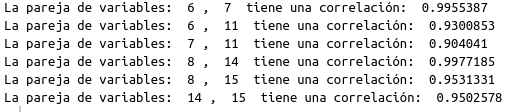
\includegraphics[scale=0.6]{./Imagenes/EDA/Regresion/correlacion_entre_variables6.png}
	\caption{Correlación entre variables después de eliminar la segunda, la novena, la cuarta, la tercera, la duodécima y la quinta.}
\end{figure}

Podemos observar que la variable 6 y 8 tienen alta correlación con otras dos variables no compartidas, por lo que podemos eliminar ambas.

\begin{figure}[H]
	\centering
	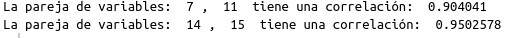
\includegraphics[scale=0.6]{./Imagenes/EDA/Regresion/correlacion_entre_variables7.png}
	\caption{Correlación entre variables después de eliminar la segunda, la novena, la cuarta, la tercera, la duodécima, la quinta, la sexta y la octava.}
\end{figure}

Finalmente nos hemos quedado con dos parejas únicamente por lo que ya no está tan claro la  eliminación de dichas variables. Vamos a parar por tanto el proceso de eliminación en este punto.

Veamos la correlación entre variables que nos queda con las que hemos decidido mantener.

\begin{figure}[H]
	\centering
	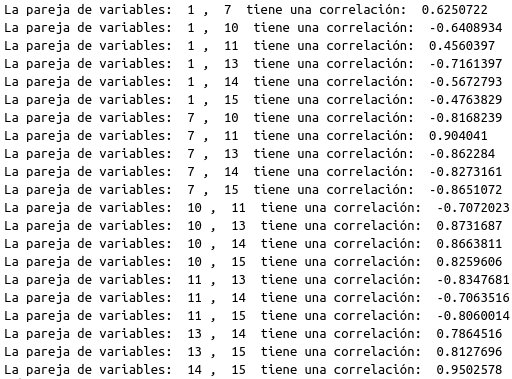
\includegraphics[scale=0.6]{./Imagenes/EDA/Regresion/correlacion_entre_variables8.png}
	\caption{Correlación entre variables después de hacer la limpieza de variables.}
\end{figure}

Finalmente por tanto nos hemos quedado con las variables 1,7,10,11,13,14 y 15.

Sobre estas variables merece la pena estudiar su correlación con la variable de salida para ver que seguimos teniendo variables que explican el comportamiento de la salida.

\begin{figure}[H]
	\centering
	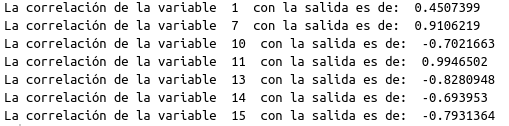
\includegraphics[scale=0.6]{./Imagenes/EDA/Regresion/correlacion_variable_salida1.png}
	\caption{Correlación de las variables no eliminadas con la variable de salida.}
\end{figure}

Podemos ver que las variables 7, 11, 13 y 15 tienen una correlación en valor absoluto mayor a $0.75$ con lo que estas variables nos van a resultar de mucho interés a la hora de realizar un modelo de regresión lineal.

Todas estas hipótesis serán contrastadas en la sección de regresión al ajustar los modelos.

\subsubsection{Valores perdidos}

En cuanto a los valores perdidos vamos a comprobar en primer lugar si tenemos valores NA.

\begin{figure}[H]
	\centering
	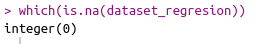
\includegraphics[scale=0.6]{./Imagenes/EDA/Regresion/valores_perdidos.png}
	\caption{Código y resultados para comprobar si tenemos valores perdidos.}
\end{figure}

Como podemos comprobar no tenemos ningún valor perdido.

\subsubsection{Outliers}

Vamos a comprobar si tenemos outliers en nuestro conjunto de datos.

En primer lugar vamos a ver un pairplot de las variables para ver si podemos distinguir algo visualmente.

\begin{figure}[H]
	\centering
	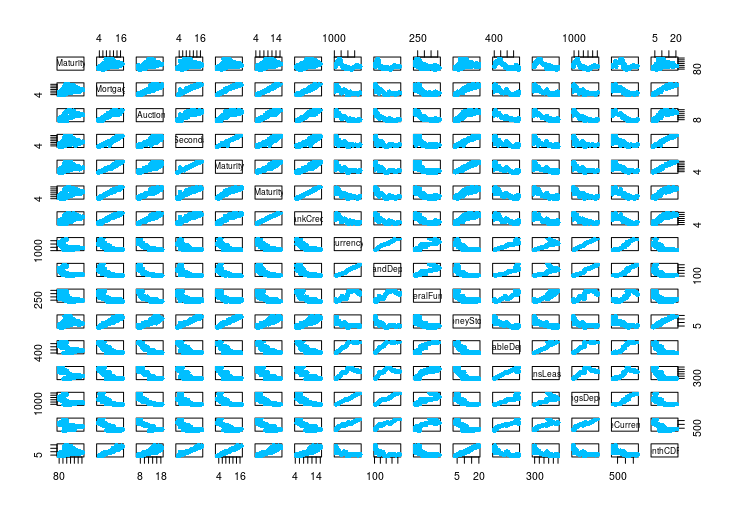
\includegraphics[scale=0.95]{./Imagenes/EDA/Regresion/pairplot_todas.png}
	\caption{Scatterplot de todas las variables dos a dos}
\end{figure}

Visualmente con tantas variables no podemos destacar ninguna anomalía. Vamos a centrarnos solamente en las variables que hemos decidido quedarnos del estudio previo.

\begin{figure}[H]
	\centering
	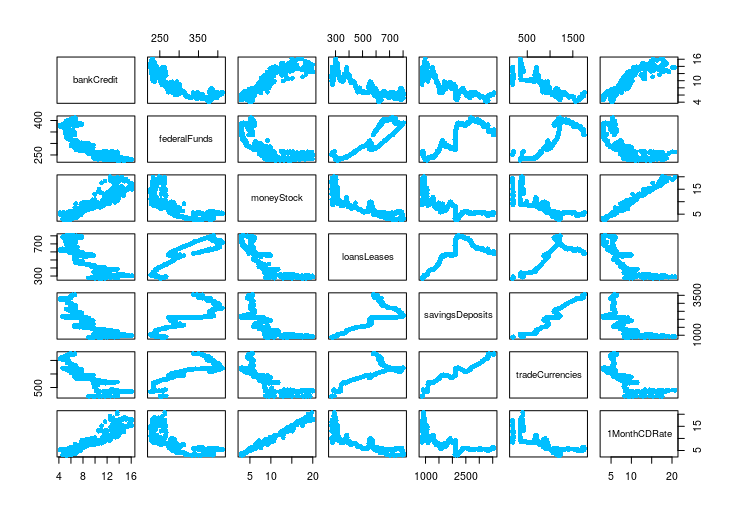
\includegraphics[scale=0.95]{./Imagenes/EDA/Regresion/pairplot_variables_seleccionadas.png}
	\caption{Scatterplot de las variables seleccionadas}
\end{figure}

Como podemos ver no podemos destacar ningún outlier en el conjunto de datos de forma visual.

De paso podemos ver que hemos hecho una selección de variables adecuada pues podemos observar una clara relación lineal con la salida.

Vamos a ver ahora un boxplot de todas las variables.

\begin{figure}[H]
	\centering
	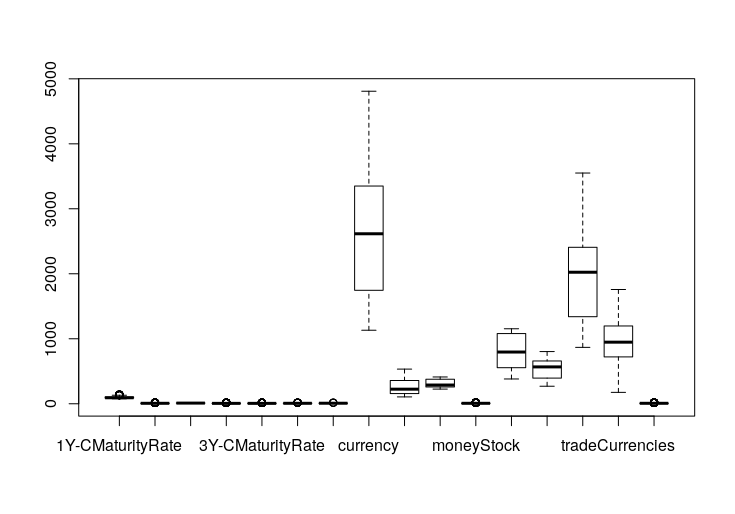
\includegraphics[scale=0.8]{./Imagenes/EDA/Regresion/boxplot_todas.png}
	\caption{Boxplot de las todas las variables}
\end{figure}

Podemos ver que por la diferencia de escalas no todas las variables son visibles. En las que podemos observar de forma adecuada podemos ver que no hay outliers que nos destaquen fuera del rango intercuartil. Por tanto podemos eliminarlas del boxplot para reducir la escala y poder ver el resto de variables.

Para el siguiente boxplot vamos a quitar las variables 8, 9, 10, 12, 13, 14 y 15.

\begin{figure}[H]
	\centering
	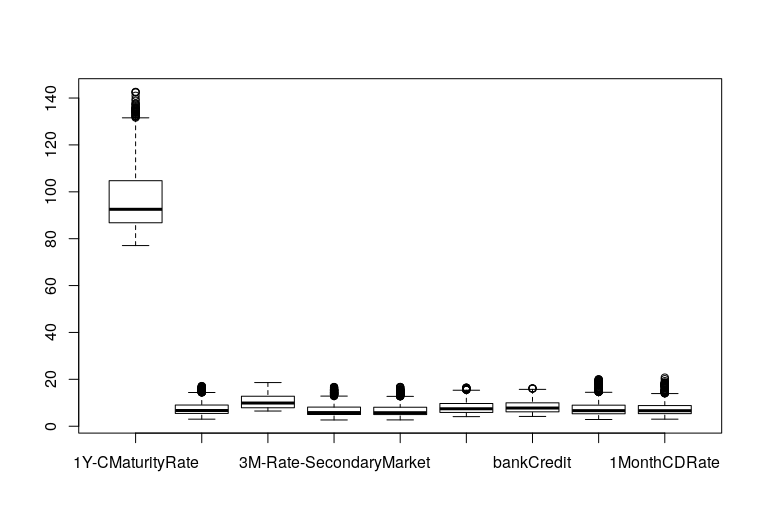
\includegraphics[scale=0.8]{./Imagenes/EDA/Regresion/boxplot_filtrado1.png}
	\caption{Boxplot quitando las variables 8, 9, 10, 12, 13, 14 y 15}
\end{figure}

Podemos observar que la primera variable tiene una escala mayor que el resto, por lo que para poder continuar la tendremos que quitar. Si observamos sus valores podemos ver que tenemos algunas anomalías por encima. Al tener tantos valores por encima no podemos decir de forma tan clara que estos valores son anómalos pues podría ser un comportamiento esperado de la variable y por tanto a priori no debemos eliminar dichos valores.

Eliminamos además la variable 1 para continuar con el estudio.

\begin{figure}[H]
	\centering
	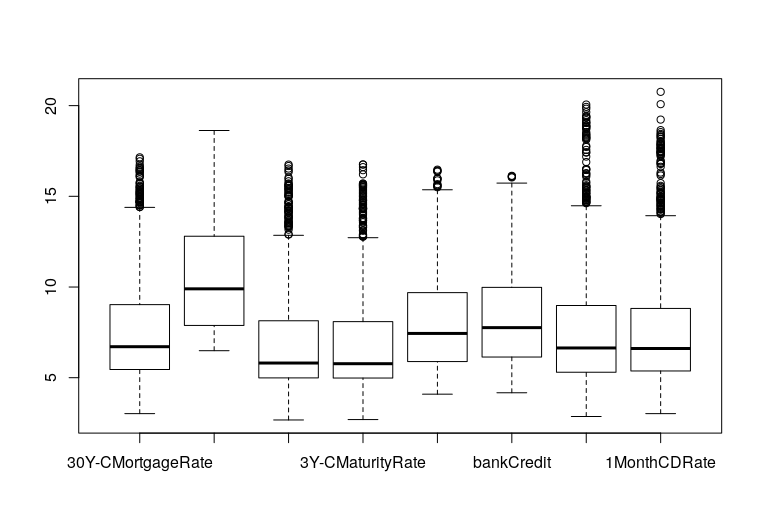
\includegraphics[scale=0.8]{./Imagenes/EDA/Regresion/boxplot_filtrado2.png}
	\caption{Boxplot quitando las variables 1, 8, 9, 10, 12, 13, 14 y 15}
\end{figure}

Podemos observar que en este último boxplot tenemos muchas más anomalías, de hecho, todas las variables poseen valores fuera del rango intercuartil menos para la segunda variable.

Podemos observar que la concentración de valores fuera de rango es muy grande por lo que no debemos eliminar dichos valores. Además este estudio es de todas las variables y no de las que hemos seleccionado para quedarnos. Veamos su boxplot.

\begin{figure}[H]
	\centering
	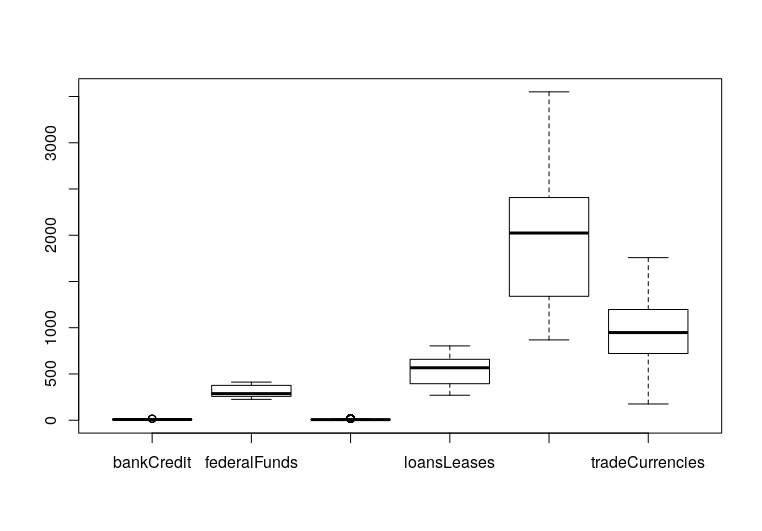
\includegraphics[scale=0.8]{./Imagenes/EDA/Regresion/boxplot_filtrado3.png}
	\caption{Boxplot manteniendo las variables seleccionadas.}
\end{figure}

Podemos ver que en las variables seleccionadas tenemos dos que poseen anomalías, vamos a estudiarlas en un boxplot aislado.

\begin{figure}[H]
	\centering
	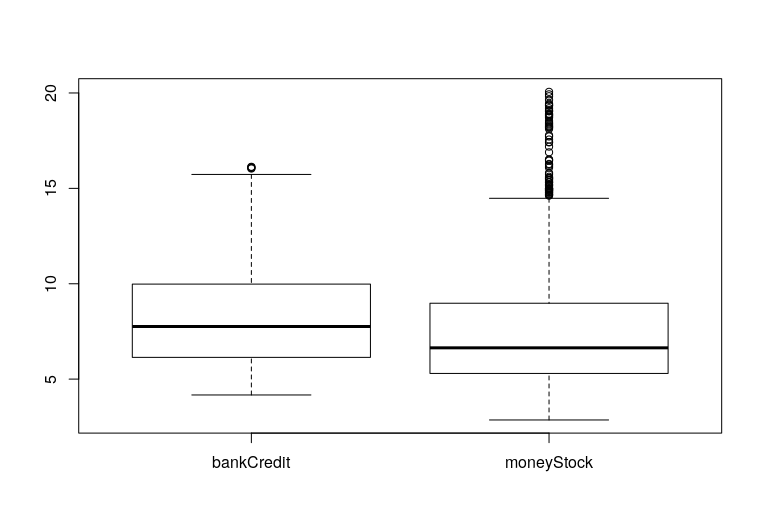
\includegraphics[scale=0.8]{./Imagenes/EDA/Regresion/boxplot_filtrado4.png}
	\caption{Boxplot de las variables que parecen tener anomalías.}
\end{figure}

Como podemos observar tenemos que la variable moneyStock tiene valores anómalos pero muy densos por lo que no debemos quitarlos. En el caso de bankCredit vamos a estudiar su scatterplot.

\begin{figure}[H]
	\centering
	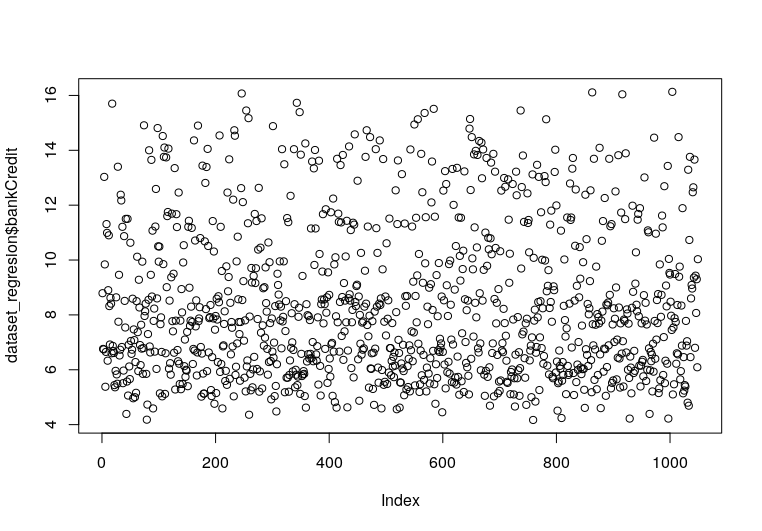
\includegraphics[scale=0.8]{./Imagenes/EDA/Regresion/scatterplot_bankCredit.png}
	\caption{ScatterPlot de la variable bankCredit}
\end{figure}

Podemos ver que las anomalías que nos encontramos no son tal pues es un conjunto distribuido de forma casi uniforme.

\subsubsection{Distribución de las variables}

Vamos a ver en primer lugar unos histogramas de las variables.

\begin{figure}[H]
	\centering
	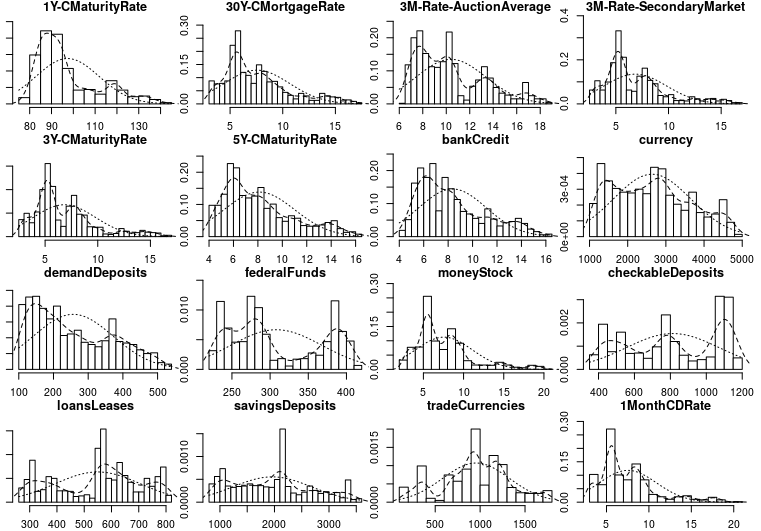
\includegraphics[scale=0.85]{./Imagenes/EDA/Regresion/histograma_todas.png}
	\caption{Histograma de todas las variables}
\end{figure}

Como podemos ver hemos acertado en el estudio previo de los estadísticos y podemos corroborar que la mayoría de variables tienen la cola derecha de su distribución más alargada. 

Podemos ver que las distribuciones no se parecen para nada a una normal de forma visual, aunque para poder estar seguros vamos a hacer un test de normalidad.

Para esto vamos a utilizar el test de Wilcoxon. Veamos los resultados.

\begin{figure}[H]
	\centering
	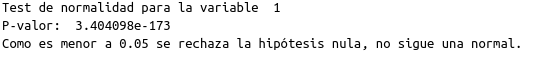
\includegraphics[scale=0.65]{./Imagenes/EDA/Regresion/test_normalidad1.png}
	\caption{Test de normalidad para la variable 1.}
\end{figure}

\begin{figure}[H]
	\centering
	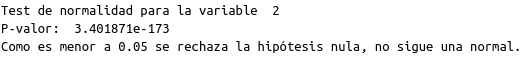
\includegraphics[scale=0.65]{./Imagenes/EDA/Regresion/test_normalidad2.png}
	\caption{Test de normalidad para la variable 2.}
\end{figure}
\begin{figure}[H]
	\centering
	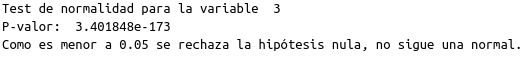
\includegraphics[scale=0.65]{./Imagenes/EDA/Regresion/test_normalidad3.png}
	\caption{Test de normalidad para la variable 3.}
\end{figure}

\begin{figure}[H]
	\centering
	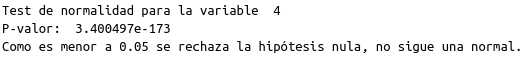
\includegraphics[scale=0.65]{./Imagenes/EDA/Regresion/test_normalidad4.png}
	\caption{Test de normalidad para la variable 4.}
\end{figure}

\begin{figure}[H]
	\centering
	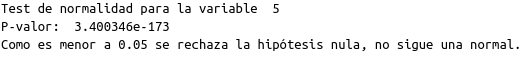
\includegraphics[scale=0.65]{./Imagenes/EDA/Regresion/test_normalidad5.png}
	\caption{Test de normalidad para la variable 5.}
\end{figure}

\begin{figure}[H]
	\centering
	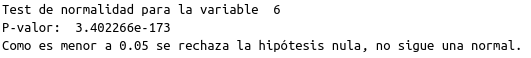
\includegraphics[scale=0.65]{./Imagenes/EDA/Regresion/test_normalidad6.png}
	\caption{Test de normalidad para la variable 6.}
\end{figure}

\begin{figure}[H]
	\centering
	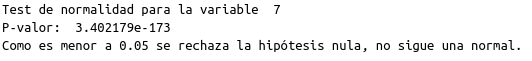
\includegraphics[scale=0.65]{./Imagenes/EDA/Regresion/test_normalidad7.png}
	\caption{Test de normalidad para la variable 7.}
\end{figure}

\begin{figure}[H]
	\centering
	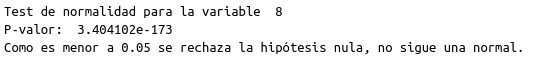
\includegraphics[scale=0.65]{./Imagenes/EDA/Regresion/test_normalidad8.png}
	\caption{Test de normalidad para la variable 8.}
\end{figure}

\begin{figure}[H]
	\centering
	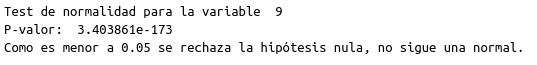
\includegraphics[scale=0.65]{./Imagenes/EDA/Regresion/test_normalidad9.png}
	\caption{Test de normalidad para la variable 9.}
\end{figure}

\begin{figure}[H]
	\centering
	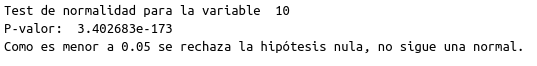
\includegraphics[scale=0.65]{./Imagenes/EDA/Regresion/test_normalidad10.png}
	\caption{Test de normalidad para la variable 10.}
\end{figure}

\begin{figure}[H]
	\centering
	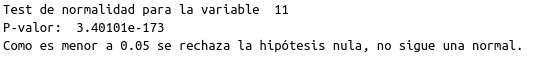
\includegraphics[scale=0.65]{./Imagenes/EDA/Regresion/test_normalidad11.png}
	\caption{Test de normalidad para la variable 11.}
\end{figure}

\begin{figure}[H]
	\centering
	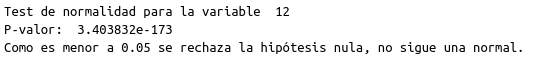
\includegraphics[scale=0.65]{./Imagenes/EDA/Regresion/test_normalidad12.png}
	\caption{Test de normalidad para la variable 12.}
\end{figure}

\begin{figure}[H]
	\centering
	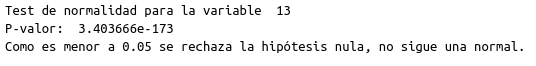
\includegraphics[scale=0.65]{./Imagenes/EDA/Regresion/test_normalidad13.png}
	\caption{Test de normalidad para la variable 13.}
\end{figure}

\begin{figure}[H]
	\centering
	\includegraphics[scale=0.65]{./Imagenes/EDA/Regresion/test_normalidad14.png}
	\caption{Test de normalidad para la variable 14.}
\end{figure}

\begin{figure}[H]
	\centering
	\includegraphics[scale=0.65]{./Imagenes/EDA/Regresion/test_normalidad15.png}
	\caption{Test de normalidad para la variable 15.}
\end{figure}

\begin{figure}[H]
	\centering
	\includegraphics[scale=0.65]{./Imagenes/EDA/Regresion/test_normalidad16.png}
	\caption{Test de normalidad para la variable 16.}
\end{figure}

Como podemos ver por los resultados del test podemos rechazar en todos los casos la hipótesis nula por lo que podemos decir que ninguna de las variables sigue una distribución normal, tal y como hemos podido ver de forma gráfica.


\subsection{Conjunto de Clasificación}

El conjunto con el que vamos a atacar el problema de clasificación es el conjunto de datos ``heart''. Vamos a analizar este conjunto de datos antes de abordar el problema.

El problema dispone de 14 variables y 270 observaciones, siendo la última la clase a la que pertenece cada instancia.

Vamos a ver los tipos de las variables.

\begin{figure}[H]
	\centering
	\includegraphics[scale=0.7]{./Imagenes/EDA/Clasificacion/tipos_variables.png}
	\caption{Tipos de las variables.}
\end{figure}

Podemos observar que todas las variables son de tipo integer, es decir, de tipo entero y que hay una variable de tipo numeric, o lo que es lo mismo, de tipo real.

Vamos a realizar el estudio del conjunto completo dividiéndolo en dos partes, la variable que nos indica la clase y el resto de variables.

\subsubsection{Estudio de los estadísticos}

\subsubsection*{Salida}

Vamos a ver los estadísticos que nos da la variable de salida o lo que es lo mismo, la clase asociada a cada instancia.

\begin{figure}[H]
	\centering
	\includegraphics[scale=0.7]{./Imagenes/EDA/Clasificacion/estadisticos_class.png}
	\caption{Estadísticos de la variable de salida.}
\end{figure}

Para poder analizar los estadísticos de esta variable tenemos que tener en cuenta que es una variable que sólo tiene dos posibles valores: 1 y 2. 

La media es $1.444444$ por lo que podemos decir que seguramente encontraremos un número mayor de instancias de la clase 1 que de la clase 2, pues si fuera al contrario la media debería ser más grande que $1.5$. Este hecho es también contrastable por el valor de la moda, o lo que es lo mismo, el valor más frecuente. La moda es $1$ por lo que ya sabemos que hay más instancias de la clase 1 que de la 2. En este caso estudiar la distribución carece de sentido por tomar únicamente dos valores, por lo que no estudiaremos la asimetría ni la curtosis.

\subsubsection*{Variable 1: Age}

Vamos a estudiar los estadísticos que nos arroja la variable.

\begin{figure}[H]
	\centering
	\includegraphics[scale=0.7]{./Imagenes/EDA/Clasificacion/estadisticos_variable1.png}
	\caption{Estadísticos de la variable 1.}
\end{figure}

En primer lugar cabe decir que esta variable es de tipo entero. Podemos ver que el intervalo en el que se mueven los valores es $[29,77]$. 

Como podemos ver la media, la mediana y la moda están muy próximas entre sí por lo que la distribución debe estar centrada. Este hecho se puede contrastar con el coeficiente de asimetría que aunque es negativo está muy cercano a $0$ lo que nos indica que la distribución es prácticamente simétrica.

En cuanto a la curtosis podemos ver que es negativa por lo que la distribución es más achatada que su normal homóloga en parámetros.

\subsubsection*{Variable 2: Sex}

Vamos a estudiar los estadísticos que nos arroja la variable.

\begin{figure}[H]
	\centering
	\includegraphics[scale=0.7]{./Imagenes/EDA/Clasificacion/estadisticos_variable2.png}
	\caption{Estadísticos de la variable 2.}
\end{figure}

Esta variable es de tipo entero y sólo puede tomar dos valores: $0$ y $1$, siendo cada uno de los números el sexo masculino o femenino. Podemos ver que la media es $0.6777778$ por lo que hay más valores de $1$ que de $0$ y por tanto debe haber un género predominante sobre el otro dentro de los datos.

Al ser una variable que sólo puede tomar dos valores no tiene sentido que estudiemos la distribución de la variable.

\subsubsection*{Variable 3: ChestPainType}

Vamos a estudiar los estadísticos que nos arroja la variable.

\begin{figure}[H]
	\centering
	\includegraphics[scale=0.7]{./Imagenes/EDA/Clasificacion/estadisticos_variable3.png}
	\caption{Estadísticos de la variable 3.}
\end{figure}

Esta variable es de tipo entero y toma valores en el intervalo $[1,4]$ indicando el tipo de dolor de pecho que posee el paciente. La media y la mediana no tienen sentido en este caso pues no son fácilmente interpretables. Al no ser algo binario no podemos establecer en qué grado aparece un valor sobre otro.

Lo que si nos puede ser útil de analizar es la moda. Podemos ver que toma valor $4$, o lo que es lo mismo, el dolor de pecho más típico es aquel que va asociado con el número $4$.

Algo que sí podemos decir sobre esta variable es que está desplazada hacia la derecha y debería de tener una cola más pesada a la derecha y más alargada a la izquierda. Esto lo podemos intuir pues la desviación típica es cercana a $1$ y por tanto el intervalo que contiene el 95\% de los datos debería de ser $[1,5]$ aproximadamente, por lo que vemos que está desplazada a la derecha con respecto al intervalo $[1,4]$.

Este dato es comprobable también por el coeficiente de asimetría que es negativo y por tanto nos indica que la distribución es asimétrica a la izquierda. En cuanto a la curtosis podemos ver que es negativa y por tanto la distribución debe ser algo más achatada que una distribución normal de mismos parámetros.

\subsubsection*{Variable 4: RestBloodPressure}

Vamos a estudiar los estadísticos que nos arroja la variable.

\begin{figure}[H]
	\centering
	\includegraphics[scale=0.7]{./Imagenes/EDA/Clasificacion/estadisticos_variable4.png}
	\caption{Estadísticos de la variable 4.}
\end{figure}

Esta es también una variable de tipo entero. Podemos ver que toma valores en el intervalo $[94, 200]$. La media y la mediana están muy próximas entre sí por lo que podemos pensar que la distribución está centrada. Por contra si miramos la moda es de $120$ por lo que podemos intuir una asimetría en la distribución.

Si miramos el coeficiente de asimetría tenemos que es positivo por lo que la distribución es asimétrica a la derecha. Esto nos indica que la cola de la derecha es algo más alargada que la de la izquierda. En cuanto a la curtosis podemos ver que es positiva por lo que la distribución es más apuntada que su distribución normal asociada de mismos parámetros.

\subsubsection*{Variable 5: SerumCholestoral}

Vamos a estudiar los estadísticos que nos arroja la variable.

\begin{figure}[H]
	\centering
	\includegraphics[scale=0.7]{./Imagenes/EDA/Clasificacion/estadisticos_variable5.png}
	\caption{Estadísticos de la variable 5.}
\end{figure}

Esta variable también es de tipo entero. El intervalo en el que toma valores es $[126,564]$. Si observamos la media y la mediana están próximas, por contra la moda es significativamente menor que ambas por lo que nos puede dar a intuir una asimetría derecha con una cola de la distribución algo más alargada.

Este hecho viene dado por el coeficiente de asimetría. Como podemos ver es positivo y además lo suficientemente grande como para que podamos decir que la asimetría es notable. Este hecho puede no ser tan sencillo de deducir a partir de los datos porque la variable es de tipo entero. Esto puede hacer que haya algunos valores más frecuentes que otros y por tanto la asimetría no sea tan evidente a través de los estadísticos básicos. 

Otro valor muy significativo es la curtosis que podemos ver que es positiva y muy grande, lo que nos está indicando que la distribución es extremadamente puntiaguda y por tanto podemos pensar que el argumento anterior (hay valores mucho más frecuentes que otros) es algo a tener en cuenta.

\subsubsection*{Variable 6: FastingBloodSugar}

Vamos a estudiar los estadísticos que nos arroja la variable.

\begin{figure}[H]
	\centering
	\includegraphics[scale=0.7]{./Imagenes/EDA/Clasificacion/estadisticos_variable6.png}
	\caption{Estadísticos de la variable 6.}
\end{figure}

La variable FastingBloodSugar es de tipo entero y sólo puede tomar dos valores: $0$ y $1$. Si vemos la media tenemos que es $0.1481481$ por lo que podemos decir que hay muchas más instancias que toman valor $0$ frente a las que toman valor $1$. El equilibrio, es decir si hubiera el mismo número de $0$ que de $1$, sería $0.5$ por lo que podemos ver el desequilibrio de valores. La moda es $0$ también por lo que corroboramos que este es el valor más frecuente.

En cuanto a la curtosis y asimetría no nos aportan más información que la ya razonada pues estamos ante una variable binaria.

\subsubsection*{Variable 7: ResElectrocardiographic}

Vamos a estudiar los estadísticos que nos arroja la variable.

\begin{figure}[H]
	\centering
	\includegraphics[scale=0.7]{./Imagenes/EDA/Clasificacion/estadisticos_variable7.png}
	\caption{Estadísticos de la variable 7.}
\end{figure}

Esta variable es también de tipo entero y podemos ver que toma valores en el intervalo $[0,2]$ por lo que sólo puede tomar los valores $0$, $1$ y $2$.La media es cercana a $1$ por lo que pueden pasar dos cosas con los valores de esta variable: la primera es que los valores que toman las 3 variables estén equilibrados y la segunda es que las ocurrencias de $0$ y $2$ estén equilibradas.

La moda es 2, cosa que podemos ver pues la media es ligeramente superior a $1$. Como tenemos una variable muy simple (sólo toma tres valores) el coeficiente de asimetría no nos da más información que la media, pudiendo corroborar que la distribución es simétrica. En cuanto a la curtosis podemos  ver que es mucho más achatada que su distribución normal asociada, por lo que podemos intuir que habrá menos ocurrencias del valor $1$ frente al $0$ y $2$.

\subsubsection*{Variable 8: MaxHeartRate}

Vamos a estudiar los estadísticos que nos arroja la variable.

\begin{figure}[H]
	\centering
	\includegraphics[scale=0.7]{./Imagenes/EDA/Clasificacion/estadisticos_variable8.png}
	\caption{Estadísticos de la variable 8.}
\end{figure}

La variable MaxHeartRate es de tipo entero. Podemos ver que toma valores en el intervalo $[71,202]$. La media y la mediana están razonablemente cercanas pero la moda es sustancialmente mayor a ambas, lo que nos está indicando que la cola izquierda debe ser algo más alargada que la derecha. Esto podríamos intentar razonarlo también calculando el intervalo en el que deberíamos encontrar el 95\% de los datos ($[103.34636,196.00924]$) pero en este caso no nos otorga mucha información.

El coeficiente de asimetría es negativo lo que nos indica una asimetría a la izquierda. La curtosis es negativa pero muy cercana a $0$ por lo que podemos decir que la distribución estará ligeramente achatada.

\subsubsection*{Variable 9: ExerciseInduced}

Vamos a estudiar los estadísticos que nos arroja la variable.

\begin{figure}[H]
	\centering
	\includegraphics[scale=0.7]{./Imagenes/EDA/Clasificacion/estadisticos_variable9.png}
	\caption{Estadísticos de la variable 9.}
\end{figure}

Esta variable es también de tipo entero y podemos ver que toma valores en el intervalo $[0,1]$ por lo que es binaria. La media es menor que $0.5$ lo que nos indica que hay más ocurrencias del valor $0$ que del valor $1$, cuestión que se refuerza al ver que la mediana y la moda son $0$.

En cuanto a la curtosis y el coeficiente de asimetría carecen de sentido al no aportar mayor información en una variable binaria.

\subsubsection*{Variable 10: Oldpeak}

Vamos a estudiar los estadísticos que nos arroja la variable.

\begin{figure}[H]
	\centering
	\includegraphics[scale=0.7]{./Imagenes/EDA/Clasificacion/estadisticos_variable10.png}
	\caption{Estadísticos de la variable 10.}
\end{figure}

Esta es la única variable del conjunto de datos que es de tipo real. Toma valores dentro del intervalo $[0,62]$ y podemos ver que la media es $8.9$. La mediana es tan solo $4$ por lo que podemos intuir que la cola derecha será muy alargada comparado con la izquierda. En cuanto a la moda podemos ver que el valor más frecuente es $0$.

Si estudiamos la curtosis y asimetría podemos ver que la distribución es muy asimétrica a la derecha, lo que sustenta el razonamiento de la cola derecha más alargada. La curtosis es positiva y muy grande por lo que podemos ver que la distribución es mucho más puntiaguda o apuntada que la distribución de una normal de mismos parámetros.

\subsubsection*{Variable 11: Slope}

Vamos a estudiar los estadísticos que nos arroja la variable.

\begin{figure}[H]
	\centering
	\includegraphics[scale=0.7]{./Imagenes/EDA/Clasificacion/estadisticos_variable11.png}
	\caption{Estadísticos de la variable 11.}
\end{figure}

La variable Slope es de tipo entero y toma valores dentro del intervalo $[1,3]$, por lo que sólo puede tomar $3$ valores distintos: $1$, $2$, y $3$. La media es $1.585185$ lo que nos indica que hay una descompensación hacia el $1$ teniendo más ocurrencias de éste valor.

Este hecho lo podemos contrastar con el valor de la moda que es $1$. En cuanto a la mediana podemos ver que es $2$ lo que nos hace pensar que aproximadamente puede haber el mismo número de ocurrencias del valor $1$ que de los valores $2$ y $3$ juntos.

El coeficiente de asimetría soporta estos razonamientos, pues es positivo indicándonos que la cola derecha es más alargada que la izquierda. En cuanto a la curtosis podemos ver que es negativa indicando que la distribución es más achatada que una normal de mismos parámetros.

\subsubsection*{Variable 12: MajorVessels}

Vamos a estudiar los estadísticos que nos arroja la variable.

\begin{figure}[H]
	\centering
	\includegraphics[scale=0.7]{./Imagenes/EDA/Clasificacion/estadisticos_variable12.png}
	\caption{Estadísticos de la variable 12.}
\end{figure}

Esta variable es de tipo entero y toma valores en el intervalo $[0,3]$, por lo que sólo puede tomar $4$ valores distintos. Podemos ver que la media está entre $0$ y $1$ lo que nos lleva a pensar que debe haber más ocurrencias de valores $0$ que del resto. La moda y la mediana corroboran esta suposición. 

La asimetría es positiva, lo que nos indica que la cola derecha debe ser más alargada que la izquierda. Por otro lado la curtosis es positiva pero no muy grande por lo que la distribución es ligeramente más apuntada que una normal de mismos parámetros.

\subsubsection*{Variable 13: Thal}

Vamos a estudiar los estadísticos que nos arroja la variable.

\begin{figure}[H]
	\centering
	\includegraphics[scale=0.7]{./Imagenes/EDA/Clasificacion/estadisticos_variable13.png}
	\caption{Estadísticos de la variable 13.}
\end{figure}

La variable Thal es de tipo entero también y toma valores en el intervalo $[3,7]$. La media es $4.696296$ y la mediana y la moda $3$. Esto nos deja pensar que la distribución será aproximadamente simétrica pues no se percibe por estos estadísticos un desbalanceo acusado. El coeficiente de asimetría, aunque positivo, posee un valor muy cercano a cero. Por otro lado la curtosis es negativa y por tanto es más achatada que su distribución normal homóloga.

\subsubsection{Estudio de la correlación de las variables}

Vamos a estudiar la correlación entre variables por si pudiéramos encontrar, como en el caso del conjunto de regresión, variables altamente correladas que se puedan eliminar.

Veamos la correlación entre las variables:

\begin{figure}[H]
	\centering
	\includegraphics[scale=0.7]{./Imagenes/EDA/Clasificacion/correlacion_entre_variables1.png}
	\caption{Correlación entre las variables sin contar la de clase.}
\end{figure}

\begin{figure}[H]
	\centering
	\includegraphics[scale=0.7]{./Imagenes/EDA/Clasificacion/correlacion_entre_variables2.png}
	\caption{Correlación entre las variables sin contar la de clase.}
\end{figure}

Como podemos observar no hay ninguna variable altamente correlada con otra, por lo que no podemos simplificar el conjunto de datos.

Este hecho puede venir de que la mayoría de variables son de tipo entero con muy pocos valores a tomar.

Veamos ahora la correlación entre las variables con la variable de clase.

\begin{figure}[H]
	\centering
	\includegraphics[scale=0.7]{./Imagenes/EDA/Clasificacion/correlacion_salida.png}
	\caption{Correlación entre las variables con la de clase.}
\end{figure}

Podemos ver que no hay variables con un alto grado de correlación con la salida. Tendremos que comprobar con el ajuste de los modelos de clasificación el desempeño que obtenemos.

\subsubsection{Valores perdidos}

Vamos a comprobar si nuestro conjunto de clasificación tiene algún valor perdido o estamos ante un conjunto limpio de missing values como en el caso de regresión.

\begin{figure}[H]
	\centering
	\includegraphics[scale=0.7]{./Imagenes/EDA/Clasificacion/valores_perdidos.png}
	\caption{Valores perdidos en el conjunto de clasificación.}
\end{figure}

Como podemos ver tenemos un conjunto sin valores perdidos, por lo que no tenemos que hacer mayores disquisiciones en este terreno.

\subsubsection{Outliers}

Vamos a observar primero un pairplot de todas las variables.

\begin{figure}[H]
	\centering
	\includegraphics[scale=0.9]{./Imagenes/EDA/Clasificacion/pairplot_todas.png}
	\caption{Pairplot de todas las variables.}
\end{figure}

En este pairplot no podemos ver demasiada información pero sí podemos intuir que hay dos tipos de variables: las que producen nubes de puntos y las que producen líneas separadas.

Vamos a verlas por separado.

\begin{figure}[H]
	\centering
	\includegraphics[scale=0.9]{./Imagenes/EDA/Clasificacion/pairplot_seleccionadas.png}
	\caption{Pairplot de las variables que producen nubes de puntos.}
\end{figure}

Aquí podemos observar las variables. Podemos ver que hay algunos puntos anómalos pero no tienen por qué representar un problema en un principio. Otra cosa que podemos ver es que estas variables no forman dos clúster separados, cosa que puede ser conflictiva al ajustar los modelos.

Vamos a ver el pairplot del resto de variables.

\begin{figure}[H]
	\centering
	\includegraphics[scale=0.9]{./Imagenes/EDA/Clasificacion/pairplot_seleccionadas2.png}
	\caption{Pairplot de las variables que forman líneas}
\end{figure}

De estos gráficos no podemos sacar demasiada información.

Vamos a hacer ahora un boxplot de todas las variables.

\begin{figure}[H]
	\centering
	\includegraphics[scale=0.7]{./Imagenes/EDA/Clasificacion/boxplot_todas.png}
	\caption{Boxplot de todas las variables.}
\end{figure}

Como podemos ver tenemos algunas anomalías o valores fuera de rango en las variables 4, 5, 6, 8 y 10.

Vamos a quitarlas para poder ver el resto.

\begin{figure}[H]
	\centering
	\includegraphics[scale=0.7]{./Imagenes/EDA/Clasificacion/boxplot_filtrado.png}
	\caption{Boxplot eliminando variables.}
\end{figure}

Como podemos ver  tenemos algunos valores que están fuera de rango y tendremos que estudiar si esto afecta a la clasificación.

Veamos también los boxplot dividiendo los valores por clases.

\begin{figure}[H]
	\centering
	\includegraphics[scale=0.6]{./Imagenes/EDA/Clasificacion/boxplot_variable1.png}
	\caption{Boxplot de la variable 1.}
\end{figure}

\begin{figure}[H]
	\centering
	\includegraphics[scale=0.6]{./Imagenes/EDA/Clasificacion/boxplot_variable2.png}
	\caption{Boxplot de la variable 2.}
\end{figure}

\begin{figure}[H]
	\centering
	\includegraphics[scale=0.6]{./Imagenes/EDA/Clasificacion/boxplot_variable3.png}
	\caption{Boxplot de la variable 3.}
\end{figure}

\begin{figure}[H]
	\centering
	\includegraphics[scale=0.6]{./Imagenes/EDA/Clasificacion/boxplot_variable4.png}
	\caption{Boxplot de la variable 4.}
\end{figure}

\begin{figure}[H]
	\centering
	\includegraphics[scale=0.6]{./Imagenes/EDA/Clasificacion/boxplot_variable5.png}
	\caption{Boxplot de la variable 5.}
\end{figure}

\begin{figure}[H]
	\centering
	\includegraphics[scale=0.6]{./Imagenes/EDA/Clasificacion/boxplot_variable6.png}
	\caption{Boxplot de la variable 6.}
\end{figure}

\begin{figure}[H]
	\centering
	\includegraphics[scale=0.6]{./Imagenes/EDA/Clasificacion/boxplot_variable7.png}
	\caption{Boxplot de la variable 7.}
\end{figure}

\begin{figure}[H]
	\centering
	\includegraphics[scale=0.6]{./Imagenes/EDA/Clasificacion/boxplot_variable8.png}
	\caption{Boxplot de la variable 8.}
\end{figure}

\begin{figure}[H]
	\centering
	\includegraphics[scale=0.6]{./Imagenes/EDA/Clasificacion/boxplot_variable9.png}
	\caption{Boxplot de la variable 9.}
\end{figure}

\begin{figure}[H]
	\centering
	\includegraphics[scale=0.6]{./Imagenes/EDA/Clasificacion/boxplot_variable10.png}
	\caption{Boxplot de la variable 10.}
\end{figure}

\begin{figure}[H]
	\centering
	\includegraphics[scale=0.6]{./Imagenes/EDA/Clasificacion/boxplot_variable11.png}
	\caption{Boxplot de la variable 11.}
\end{figure}

\begin{figure}[H]
	\centering
	\includegraphics[scale=0.6]{./Imagenes/EDA/Clasificacion/boxplot_variable12.png}
	\caption{Boxplot de la variable 12.}
\end{figure}

\begin{figure}[H]
	\centering
	\includegraphics[scale=0.6]{./Imagenes/EDA/Clasificacion/boxplot_variable13.png}
	\caption{Boxplot de la variable 13.}
\end{figure}

En este problema no es tan sencillo decir que un valor es anómalo frente al resto. Al ser la mayoría de variables de tipo entero y con pocos valores simplemente puede que se esté dando el caso de que tengamos una concentración de valores mayor de uno de los posibles valores frente al resto y esto haga que los demás se consideren anómalos en el boxplot por cómo resulta el cálculo del rango intercuartil.

\subsubsection{Distribución de las variables}

Vamos a estudiar la distribución de las variables con un histograma de todas las variables.

\begin{figure}[H]
	\centering
	\includegraphics[scale=0.9]{./Imagenes/EDA/Clasificacion/histograma_todas.png}
	\caption{Histograma de todas las variables.}
\end{figure}

En primer lugar cabe decir que los histogramas de las variables que toman muy pocos valores carecen de sentido pues van a salir degenerados. Este es el caso de las variables Sex, ChestPainType, FastingBloodSugar, etc.

En un estudio visual podemos ver que hay algunas variables que puede que tengan una distribución normal. Vamos a ver si podemos decir algo acerca de esto con un test de normalidad.

\begin{figure}[H]
	\centering
	\includegraphics[scale=0.6]{./Imagenes/EDA/Clasificacion/test_normalidad1.png}
	\caption{Test de normalidad para la variable 1.}
\end{figure}

\begin{figure}[H]
	\centering
	\includegraphics[scale=0.6]{./Imagenes/EDA/Clasificacion/test_normalidad2.png}
	\caption{Test de normalidad para la variable 2.}
\end{figure}

\begin{figure}[H]
	\centering
	\includegraphics[scale=0.6]{./Imagenes/EDA/Clasificacion/test_normalidad3.png}
	\caption{Test de normalidad para la variable 3.}
\end{figure}

\begin{figure}[H]
	\centering
	\includegraphics[scale=0.6]{./Imagenes/EDA/Clasificacion/test_normalidad4.png}
	\caption{Test de normalidad para la variable 4.}
\end{figure}

\begin{figure}[H]
	\centering
	\includegraphics[scale=0.6]{./Imagenes/EDA/Clasificacion/test_normalidad5.png}
	\caption{Test de normalidad para la variable 5.}
\end{figure}

\begin{figure}[H]
	\centering
	\includegraphics[scale=0.6]{./Imagenes/EDA/Clasificacion/test_normalidad6.png}
	\caption{Test de normalidad para la variable 6.}
\end{figure}

\begin{figure}[H]
	\centering
	\includegraphics[scale=0.6]{./Imagenes/EDA/Clasificacion/test_normalidad7.png}
	\caption{Test de normalidad para la variable 7.}
\end{figure}

\begin{figure}[H]
	\centering
	\includegraphics[scale=0.6]{./Imagenes/EDA/Clasificacion/test_normalidad8.png}
	\caption{Test de normalidad para la variable 8.}
\end{figure}

\begin{figure}[H]
	\centering
	\includegraphics[scale=0.6]{./Imagenes/EDA/Clasificacion/test_normalidad9.png}
	\caption{Test de normalidad para la variable 9.}
\end{figure}

\begin{figure}[H]
	\centering
	\includegraphics[scale=0.6]{./Imagenes/EDA/Clasificacion/test_normalidad10.png}
	\caption{Test de normalidad para la variable 10.}
\end{figure}

\begin{figure}[H]
	\centering
	\includegraphics[scale=0.6]{./Imagenes/EDA/Clasificacion/test_normalidad11.png}
	\caption{Test de normalidad para la variable 11.}
\end{figure}

\begin{figure}[H]
	\centering
	\includegraphics[scale=0.6]{./Imagenes/EDA/Clasificacion/test_normalidad12.png}
	\caption{Test de normalidad para la variable 12.}
\end{figure}

\begin{figure}[H]
	\centering
	\includegraphics[scale=0.6]{./Imagenes/EDA/Clasificacion/test_normalidad13.png}
	\caption{Test de normalidad para la variable 13.}
\end{figure}

\begin{figure}[H]
	\centering
	\includegraphics[scale=0.6]{./Imagenes/EDA/Clasificacion/test_normalidad14.png}
	\caption{Test de normalidad para la variable 14.}
\end{figure}

Como podemos comprobar, en todos los casos tenemos p-valores más pequeños que $0.05$ por lo que en todos los casos rechazamos la hipótesis nula y por tanto descartamos que ninguna de las variables siga una distribución normal.

\section{Regresión: Treasury}

En esta sección vamos a abordar el problema de regresión dado por el conjunto de datos Treasury.

Ya hemos analizado previamente las características del conjunto de datos y hemos hecho hipótesis de variables que podríamos quitar. Vamos a ver en esta sección si dichas hipótesis estaban fundamentadas o no.

\subsection{Regresión lineal simple}

En esta sección se va a resolver el primero de los apartados del problema de regresión. Para ello lo que se ha realizado es generar todos los modelos de regresión posibles con una sola variable para el problema dado.

Como tenemos 16 variables en total en el conjunto de datos tendremos por tanto 15 modelos al final. De entre estos se nos ha pedido que escojamos los 5 mejores. Vamos a ver los resultados que los modelos nos otorgan y vamos a escoger en consecuencia los 5 mejores modelos.

\begin{figure}[H]
	\centering 
	\includegraphics[scale=0.55]{./Imagenes/Regresion/regresor_1va1.png}
	\caption{Regresor con la variable 1Y-CMaturityRate.}
\end{figure}

\begin{figure}[H]
	\centering 
	\includegraphics[scale=0.55]{./Imagenes/Regresion/regresor_1va2.png}
	\caption{Regresor con la variable 30Y-CMortgageRate.}
\end{figure}

\begin{figure}[H]
	\centering 
	\includegraphics[scale=0.55]{./Imagenes/Regresion/regresor_1va3.png}
	\caption{Regresor con la variable 3M-Rate-AuctionAverage.}
\end{figure}

\begin{figure}[H]
	\centering 
	\includegraphics[scale=0.55]{./Imagenes/Regresion/regresor_1va4.png}
	\caption{Regresor con la variable 3M-Rate-SecondaryMarket.}
\end{figure}

\begin{figure}[H]
	\centering 
	\includegraphics[scale=0.55]{./Imagenes/Regresion/regresor_1va5.png}
	\caption{Regresor con la variable 3Y-CMaturityRate.}
\end{figure}

\begin{figure}[H]
	\centering 
	\includegraphics[scale=0.55]{./Imagenes/Regresion/regresor_1va6.png}
	\caption{Regresor con la variable 5Y-CMaturityRate.}
\end{figure}

\begin{figure}[H]
	\centering 
	\includegraphics[scale=0.55]{./Imagenes/Regresion/regresor_1va7.png}
	\caption{Regresor con la variable bankCredit.}
\end{figure}

\begin{figure}[H]
	\centering 
	\includegraphics[scale=0.55]{./Imagenes/Regresion/regresor_1va8.png}
	\caption{Regresor con la variable currency.}
\end{figure}

\begin{figure}[H]
	\centering 
	\includegraphics[scale=0.55]{./Imagenes/Regresion/regresor_1va9.png}
	\caption{Regresor con la variable demandDeposits.}
\end{figure}

\begin{figure}[H]
	\centering 
	\includegraphics[scale=0.55]{./Imagenes/Regresion/regresor_1va10.png}
	\caption{Regresor con la variable federalFunds.}
\end{figure}

\begin{figure}[H]
	\centering 
	\includegraphics[scale=0.55]{./Imagenes/Regresion/regresor_1va11.png}
	\caption{Regresor con la variable moneyStock.}
\end{figure}

\begin{figure}[H]
	\centering 
	\includegraphics[scale=0.55]{./Imagenes/Regresion/regresor_1va12.png}
	\caption{Regresor con la variable checkableDeposits.}
\end{figure}

\begin{figure}[H]
	\centering 
	\includegraphics[scale=0.55]{./Imagenes/Regresion/regresor_1va13.png}
	\caption{Regresor con la variable loansLeases.}
\end{figure}

\begin{figure}[H]
	\centering 
	\includegraphics[scale=0.55]{./Imagenes/Regresion/regresor_1va14.png}
	\caption{Regresor con la variable savingsDeposits.}
\end{figure}

\begin{figure}[H]
	\centering 
	\includegraphics[scale=0.55]{./Imagenes/Regresion/regresor_1va15.png}
	\caption{Regresor con la variable tradeCurrencies.}
\end{figure}

Para poder discernir los modelos que mejor desempeño tienen vamos a analizar los valores de $R^2$ ajustado.

Según los valores que hemos obtenido los 5 mejores modelos son:

\begin{table}[H]
	\centering
	\begin{tabular}{|c|c|}
		\hline
		\textbf{Variable}       & \textbf{$R^2$ ajustado} \\ \hline
		moneyStock              & 0.9893                  \\ \hline
		3Y-CMaturityRate        & 0.9835                  \\ \hline
		3M-Rate-SecondaryMarket & 0.9807                  \\ \hline
		30Y-CMortgageRate       & 0.9551                  \\ \hline
		5Y-CMaturityRate        & 0.8794                  \\ \hline
	\end{tabular}
\end{table}

Aquí podemos intuir que estas variables van a ser extremadamente importantes en el problema de regresión pues por ellas solas obtienen ya un buen resultado.

Vamos a ver las gráficas que obtienen y su línea predicha.

\begin{figure}[H]
	\centering 
	\includegraphics[scale=0.65]{./Imagenes/Regresion/abline_moneyStock.png}
	\caption{Conjunto de datos y la línea obtenida por el modelo con la variable moneyStock.}
\end{figure}

\begin{figure}[H]
	\centering 
	\includegraphics[scale=0.65]{./Imagenes/Regresion/abline_3Y_CMaturityRate.png}
	\caption{Conjunto de datos y la línea obtenida por el modelo con la variable 3Y-CMaturityRate.}
\end{figure}

\begin{figure}[H]
	\centering 
	\includegraphics[scale=0.65]{./Imagenes/Regresion/abline_3M_Rate_SecondaryMarket.png}
	\caption{Conjunto de datos y la línea obtenida por el modelo con la variable 3M-Rate-SecondaryMarket.}
\end{figure}

\begin{figure}[H]
	\centering 
	\includegraphics[scale=0.65]{./Imagenes/Regresion/abline_30Y_CMortgageRate.png}
	\caption{Conjunto de datos y la línea obtenida por el modelo con la variable 30Y-CMortgageRate.}
\end{figure}

\begin{figure}[H]
	\centering 
	\includegraphics[scale=0.65]{./Imagenes/Regresion/abline_5Y_CMaturityRate.png}
	\caption{Conjunto de datos y la línea obtenida por el modelo con la variable 5Y-CMaturityRate.}
\end{figure}

Como podemos observar el ajuste es muy bueno en las 4 primeras variables y en la segunda algo peor sobre todo cuanto mayores son los valores de la variable de salida.

El error cometido por los modelos coincide en la ordenación del $R^2$ ajustado.

Los modelos de una sola variable ya nos proporcionan unos resultados realmente buenos teniendo el mejor de ellos un $R^2$ ajustado de $0.9893$, lo que nos va a dar un margen de mejora realmente escaso. Aún así vamos a continuar con modelos más complejos para ver si podemos mejorar este resultado.

\subsection{Regresión lineal múltiple}

En este apartado vamos a estudiar los modelos de regresión lineal múltiple. Para empezar esta sección vamos a ir de más a menos empezando con un modelo que emplee todas las variable y luego iremos eliminando las variables de menor calidad hasta obtener un modelo simple con un buen rendimiento.

\begin{figure}[H]
	\centering 
	\includegraphics[scale=0.65]{./Imagenes/Regresion/regresion_multiple1.png}
	\caption{Resultados para el modelo con todas las variables.}
\end{figure}

Como podemos ver tenemos varias variables que proporcionan malos resultados o que no aportan información como la variable federalFunds.

En cuanto al $R^2$ ajustado podemos ver que es $0.995$, lo que nos está indicando que el modelo es de mucha calidad en cuanto al ajuste, pero no podemos olvidar que el mejor resultado de los modelos de una única variable fue $0.9893$.

Vamos a eliminar las variables de mala calidad para el ajuste como por ejemplo la variable federalFunds.

\begin{figure}[H]
	\centering 
	\includegraphics[scale=0.65]{./Imagenes/Regresion/regresion_multiple2.png}
	\caption{Resultados eliminando la variable federalFunds.}
\end{figure}

Podemos ver que incluso el $R^2$ ajustado ha subido ligeramente. Esto no es porque el modelo haya mejorado su regresión eliminando una variable, sino porque el $R^2$ ajustado se calcula también en base al número de variables que participan en el modelo y al eliminar una podemos haber producido el aumento.

\begin{figure}[H]
	\centering 
	\includegraphics[scale=0.65]{./Imagenes/Regresion/regresion_multiple3.png}
	\caption{Resultados eliminando la variable federalFunds y 3M-Rate-AuctionAverage.}
\end{figure}

Podemos ver que el valor de $R^2$ ajustado no ha variado al eliminar la variable 3M-Rate-AuctionAverage. Vamos a continuar eliminando la variable 3M-Rate-SecondaryMarket.

\begin{figure}[H]
	\centering 
	\includegraphics[scale=0.65]{./Imagenes/Regresion/regresion_multiple4.png}
	\caption{Resultados eliminando la variable federalFunds, 3M-Rate-AuctionAverage y 3M-Rate-SecondaryMarket.}
\end{figure}

Seguimos sin bajar en la bondad del ajuste, por lo que sabemos que estamos yendo en la buena dirección. Vamos a eliminar ahora la variable 5Y-CMaturityRate.

\begin{figure}[H]
	\centering 
	\includegraphics[scale=0.6]{./Imagenes/Regresion/regresion_multiple5.png}
	\caption{Resultados eliminando la variable federalFunds, 3M-Rate-AuctionAverage, 3M-Rate-SecondaryMarket y 5Y-CMaturityRate.}
\end{figure}

Como podemos ver hemos bajado ligeramente la bondad del ajuste al eliminar la última variable, pero la reducción ha sido tan baja que no es apreciable. Seguimos teniendo una variable que no está dando demasiado peso en el modelo y por tanto podríamos pensar en eliminarla. Vamos a ver qué ocurre cuando eliminamos la variable demandDeposits.

\begin{figure}[H]
	\centering 
	\includegraphics[scale=0.6]{./Imagenes/Regresion/regresion_multiple6.png}
	\caption{Resultados eliminando la variable federalFunds, 3M-Rate-AuctionAverage, 3M-Rate-SecondaryMarket, 5Y-CMaturityRate y demandDeposits.}
\end{figure}

Vemos que seguimos manteniendo el ajuste. Vamos a ver si eliminamos ahora bankCredit.

\begin{figure}[H]
	\centering 
	\includegraphics[scale=0.6]{./Imagenes/Regresion/regresion_multiple7.png}
	\caption{Resultados eliminando la variable federalFunds, 3M-Rate-AuctionAverage, 3M-Rate-SecondaryMarket, 5Y-CMaturityRate, demandDeposits y bankCredit.}
\end{figure}

Podemos ver que ahora la variable savingsDeposits nos está dando un ajuste un poco peor que el resto. Como no hemos reducido el rendimiento del modelo podemos probar a eliminar esta variable para ver si empeoramos el ajuste.

\begin{figure}[H]
	\centering 
	\includegraphics[scale=0.6]{./Imagenes/Regresion/regresion_multiple8.png}
	\caption{Resultados eliminando la variable federalFunds, 3M-Rate-AuctionAverage, 3M-Rate-SecondaryMarket, 5Y-CMaturityRate, demandDeposits, bankCredit y savingsDeposits.}
\end{figure}

Podemos ver que hemos bajado un poco en el ajuste pero hemos reducido considerablemente la complejidad del modelo eliminando muchas variables. Podemos intentar eliminar alguna variable más aunque ya estamos en p-valores muy bajos, por lo que es probable que al eliminar alguna variable más ya si reduzcamos el desempeño del modelo de forma significativa. 

Si comparamos los p-valores de las variables la siguiente candidata a ser eliminada del modelo sería currency. Vamos a ver los resultados que obtenemos si la eliminamos.

\begin{figure}[H]
	\centering 
	\includegraphics[scale=0.6]{./Imagenes/Regresion/regresion_multiple9.png}
	\caption{Resultados eliminando la variable federalFunds, 3M-Rate-AuctionAverage, 3M-Rate-SecondaryMarket, 5Y-CMaturityRate, demandDeposits, bankCredit, savingsDeposits y currency.}
\end{figure}

Seguimos teniendo un modelo con buenos resultados y ahora podemos ver que la variable que empeora el resultado del modelo debería ser loansLeases, por lo que podemos eliminarla y ver si obtenemos resultados mucho peores o mantenemos la línea de ajuste.

\begin{figure}[H]
	\centering 
	\includegraphics[scale=0.6]{./Imagenes/Regresion/regresion_multiple10.png}
	\caption{Resultados eliminando la variable federalFunds, 3M-Rate-AuctionAverage, 3M-Rate-SecondaryMarket, 5Y-CMaturityRate, demandDeposits, bankCredit, savingsDeposits, currency y loansLeases.}
\end{figure}

El ajuste no ha empeorado y de nuevo tenemos una situación en la que no podemos eliminar a priori ninguna de las variables. La que tiene un p-valor más grande es checkableDeposits.

\begin{figure}[H]
	\centering 
	\includegraphics[scale=0.6]{./Imagenes/Regresion/regresion_multiple11.png}
	\caption{Resultados eliminando la variable federalFunds, 3M-Rate-AuctionAverage, 3M-Rate-SecondaryMarket, 5Y-CMaturityRate, demandDeposits, bankCredit, savingsDeposits, currency, loansLeases y checkableDeposits.}
\end{figure}

El ajuste no ha empeorado casi el modelo por lo que vamos a continuar reduciendo el problema. Podemos ver que de todas las variables iniciales, las que explican el problema y lo resuelven son muchas menos. Vamos a eliminar la variable 30Y-CMortgageRate.

\begin{figure}[H]
	\centering 
	\includegraphics[scale=0.6]{./Imagenes/Regresion/regresion_multiple12.png}
	\caption{Resultados eliminando la variable federalFunds, 3M-Rate-AuctionAverage, 3M-Rate-SecondaryMarket, 5Y-CMaturityRate, demandDeposits, bankCredit, savingsDeposits, currency, loansLeases, checkableDeposits y 30Y-CMortgageRate.}
\end{figure}

Estamos empeorando en el ajuste de forma muy ligera pero merece la pena por la tremenda simplificación del problema. Como podemos ver todavía tenemos las dos variables que mejor ajuste han producido por sí solas.

Vamos a eliminar la variable con un p-valor mayor, que en este caso es 1Y-CMaturityRate.

\begin{figure}[H]
	\centering 
	\includegraphics[scale=0.6]{./Imagenes/Regresion/regresion_multiple13.png}
	\caption{Resultados eliminando la variable federalFunds, 3M-Rate-AuctionAverage, 3M-Rate-SecondaryMarket, 5Y-CMaturityRate, demandDeposits, bankCredit, savingsDeposits, currency, loansLeases, checkableDeposits, 30Y-CMortgageRate y 1Y-CMaturityRate.}
\end{figure}

Hemos obtenido un modelo mucho más reducido que el inicial que tiene un $R^2$ ajustado de $0.9942$, lo cual es más que lo que hemos obtenido en la mejor de las regresiones lineales simples. Hemos disminuido un poco el rendimiento, pues inicialmente partíamos de un modelo que tenía un $R^2$ ajustado de $0.9951$ pero he decidido sacrificar un poco de rendimiento (hemos bajado sólo $0.001$ en el $R^2$ ajustado) por simplificar enormemente el modelo.

Claramente el modelo obtenido es superior al modelo simple pues mejoramos el rendimiento únicamente empleando dos variables más. Recordemos que el mejor rendimiento lo obtuvimos con la variable moneyStock que nos dio un $R^2$ ajustado de $0.9893$ y hemos subido el rendimiento a $0.9942$. Si queremos primar la simplicidad del modelo frente a un mejor rendimiento está claro que el modelo de una única variable es suficientemente bueno. Por contra si queremos un poco más de rendimiento a costa de aumentar ligeramente la complejidad de la solución podemos optar por el modelo de regresión múltiple de 3 variables que hemos generado.

Recordemos que en la fase de EDA hicimos suposiciones sobre las variables que podíamos eliminar. En el estudio exploratorio concluimos que a priori parecían interesantes las variables 7,10,11,13,14 y 15. Veamos el desempeño de dicho modelo.

\begin{figure}[H]
	\centering 
	\includegraphics[scale=0.6]{./Imagenes/Regresion/regresion_multiple14.png}
	\caption{Resultados con las variables escogidas en el EDA.}
\end{figure}

Podemos ver que el rendimiento del modelo es incluso peor que el que nos proporciona la variable moneyStock por sí sola por lo que este modelo no es una buena opción.

En cuanto a interacciones no lineales podemos probar con el modelo simple de 3 variables que hemos obtenido haciendo algunas transformaciones no lineales, pero debemos tener presente que es complicado obtener resultados mucho mejores que los que ya tenemos.

\begin{figure}[H]
	\centering 
	\includegraphics[scale=0.6]{./Imagenes/Regresion/regresion_multiple15.png}
	\caption{Regresión con interacciones no lineales.}
\end{figure}

Como podemos ver por la fórmula que estamos aplicando estamos considerando todas las posibles interacciones cuadráticas que implican las 3 variables consideradas en el último modelo. Como podemos ver no obtenemos una mejora significativa, pues mejoramos el $R^2$ ajustado solamente $0.0001$ por lo tanto no merece la pena.

\subsection{Algoritmo k-NN para regresión}

En esta sección vamos a emplear el algoritmo KNN para regresión. Para ello vamos a aplicarlo primero con todas las variables, después con la que mejor resultado nos ha dado en los modelos de regresión simple y posteriormente con la mejor fórmula del modelo de regresión múltiple.

Para comparar los algoritmos vamos a emplear el error en predicción en train y en test por cada fold y en media. A priori además no sabemos el valor que debemos emplear para K, por lo que vamos a hacer un estudio al respecto para elegir bien dicho valor variándolo entre 3 y 55 a saltos de 2.

\begin{figure}[H]
	\centering 
	\includegraphics[scale=0.6]{./Imagenes/Regresion/knn1.png}
	\caption{Error en test del modelo KNN con todas las variables.}
\end{figure}

Podemos ver claramente que el valor de K para el que se obtiene el menor error es para $K=5$ donde obtenemos de media $0.04609969$ de error en los folds. Si estudiamos el error por fold vemos que tenemos los siguientes números:

\begin{table}[H]
	\centering
	\begin{tabular}{|c|c|}
		\hline
		\textbf{Folds} & \textbf{Error} \\ \hline
		1              & 0.07921098     \\ \hline
		2              & 0.05298160     \\ \hline
		3              & 0.02544653     \\ \hline
		4              & 0.04156857     \\ \hline
		5              & 0.03129077     \\ \hline
	\end{tabular}
\end{table}

En cuanto al error en el train para cada valor de K obtenemos la siguiente gráfica:

\begin{figure}[H]
	\centering 
	\includegraphics[scale=0.6]{./Imagenes/Regresion/knn2.png}
	\caption{Error en train del modelo KNN con todas las variables.}
\end{figure}

Podemos ver que el menor error se comete con $K=3$ donde obtenemos un error medio de $0.00509912$ en la validación cruzada. El error cometido por cada fold es:

\begin{table}[H]
	\centering
	\begin{tabular}{|c|c|}
		\hline
		\textbf{Fold} & \textbf{Error} \\ \hline
		1              & 0.005395550     \\ \hline
		2              & 0.004238368     \\ \hline
		3              & 0.004765470     \\ \hline
		4              & 0.005374334     \\ \hline
		5              & 0.005721879     \\ \hline
	\end{tabular}
\end{table}

Vamos a ver ahora el error que se comete empleando la mejor variable de los modelos lineales simples.

\begin{figure}[H]
	\centering 
	\includegraphics[scale=0.6]{./Imagenes/Regresion/knn3.png}
	\caption{Error en test del modelo KNN con la variable moneyStock.}
\end{figure}

Podemos ver en esta gráfica que el modelo con una sola variable es muy dependiente del valor de K. El mejor valor que podemos tomar para este parámetro es $21$ ya que es el que menos error nos da en media en la validación cruzada. El error cometido en media en el test es $0.1237461$ y por cada fold:

\begin{table}[H]
	\centering
	\begin{tabular}{|c|c|}
		\hline
		\textbf{Fold} & \textbf{Error} \\ \hline
		1              & 0.15658084     \\ \hline
		2              & 0.16779980     \\ \hline
		3              & 0.10178984     \\ \hline
		4              & 0.10885809     \\ \hline
		5              & 0.08370183     \\ \hline
	\end{tabular}
\end{table}

Veamos el error en el train:

\begin{figure}[H]
	\centering 
	\includegraphics[scale=0.6]{./Imagenes/Regresion/knn4.png}
	\caption{Error en train del modelo KNN con la variable moneyStock.}
\end{figure}

Como podemos ver en el caso del train el mejor resultado de error se obtiene para el valor de $K=3$. En este caso se comete un error de $0.06193327$. El error por folds es:

\begin{table}[H]
	\centering
	\begin{tabular}{|c|c|}
		\hline
		\textbf{Fold} & \textbf{Error} \\ \hline
		1              & 0.05902647     \\ \hline
		2              & 0.05254069     \\ \hline
		3              & 0.06674650     \\ \hline
		4              & 0.06400127     \\ \hline
		5              & 0.06735141     \\ \hline
	\end{tabular}
\end{table}

Vamos a ver ahora el desempeño que tiene el modelo KNN con las tres variables que tomamos finalmente en el estudio de regresión múltiple.

\begin{figure}[H]
	\centering 
	\includegraphics[scale=0.6]{./Imagenes/Regresion/knn5.png}
	\caption{Error en test del modelo KNN con las variables 3Y-CMaturityRate, moneyStock y tradeCurrencies.}
\end{figure}

Podemos ver que el menor valor de error se produce con el valor $K=9$ siendo dicho error en media $0.05378016$. Si analizamos el error por fold podemos ver que obtenemos los siguientes resultados:

\begin{table}[H]
	\centering
	\begin{tabular}{|c|c|}
		\hline
		\textbf{Fold} & \textbf{Error} \\ \hline
		1              & 0.08178329     \\ \hline
		2              & 0.06936034     \\ \hline
		3              & 0.03370024     \\ \hline
		4              & 0.04640869     \\ \hline
		5              & 0.03764825     \\ \hline
	\end{tabular}
\end{table}

Veamos ahora el mejor valor de K según el error cometido en el train y comparemos finalmente los modelos.

El error cometido en media en el train según el valor de K es el siguiente:

\begin{figure}[H]
	\centering 
	\includegraphics[scale=0.6]{./Imagenes/Regresion/knn6.png}
	\caption{Error en train del modelo KNN con las variables 3Y-CMaturityRate, moneyStock y tradeCurrencies.}
\end{figure}

Podemos ver que el menor error se comete para el valor de K igual a $3$, donde se comete en media un error de $0.01161164$. Si analizamos el error por folds obtenemos los siguientes resultados:

\begin{table}[H]
	\centering
	\begin{tabular}{|c|c|}
		\hline
		\textbf{Fold} & \textbf{Error} \\ \hline
		1              & 0.00975913     \\ \hline
		2              & 0.01180357     \\ \hline
		3              & 0.01163929     \\ \hline
		4              & 0.01197810     \\ \hline
		5              & 0.01287809     \\ \hline
	\end{tabular}
\end{table}

Vamos a comparar por tanto los modelos obtenidos. Para esta comparación vamos a tanto el error por folds en el test como el error medio cometido en los mismos. Se nos podría plantear en esta sección el dilema de si emplear el error en train o en test para hacer la comparativa o ambos incluso. Desde un punto de vista objetivo debemos usar el error cometido sobre el test. Nosotros estamos suponiendo que disponemos de datos que conocemos (los del train) y estamos entrenando el modelo con ellos para luego evaluarlo con unos datos nuevos simulando que son datos desconocidos para nosotros como si nos llegasen en una aplicación real del modelo. Por tanto lo más consistente es evaluarlo empleando el error cometido en el test.

Veamos la siguiente tabla:

\begin{table}[H]
	\centering
	\begin{tabular}{|c|c|c|c|}
		\hline
		\textbf{Folds}       & \textbf{Error modelo todas} & \textbf{Error moneyStock} & \textbf{Error modelo tres variables} \\ \hline
		1                    & 0.07921098                  & 0.15658084                & 0.08178329                           \\ \hline
		2                    & 0.05298160                  & 0.16779980                & 0.06936034                           \\ \hline
		3                    & 0.02544653                  & 0.10178984                & 0.03370024                           \\ \hline
		4                    & 0.04156857                  & 0.10885809                & 0.04640869                           \\ \hline
		5                    & 0.03129077                  & 0.08370783                & 0.03764825                           \\ \hline
		\textbf{Error medio} & 0.04609969                  & 0.1237461                 & 0.05378016                           \\ \hline
	\end{tabular}
\end{table}

Podemos comprobar que el peor modelo en cuanto a error cometido es el modelo que emplea una única variable para el ajuste con KNN. Este modelo comete un error mayor en todos los folds comparado con los otros dos modelos del KNN, lo cual se hace evidente también en el error medio como era de esperar.

Entre el modelo de tres variables y el modelo que hace uso de todas podemos ver que el modelo que comete un error menor es el modelo que emplea todas las variables. Esto es algo lógico pues lo vimos también en el ajuste de regresión lineal múltiple que con todas las variables obteníamos un buen resultado. En ese caso primamos la simplicidad que ganábamos frente a una pérdida de rendimiento menor. Si observamos la diferencia de errores cometidos es de $0.00768047$ en el error medio, lo cual es prácticamente insignificante y por tanto es muy lógico pensar que el modelo más simple de tres variables es una mejor opción que el modelo que hace uso de todas.

\subsection{Test de significancia entre algoritmos}

Queremos ver ahora si los algoritmos son significativamente diferentes por los resultados que nos han arrojado. Para ello primero vamos a hacer una comparativa entre los algoritmos KNN y regresión lineal múltiple con la configuración de todas las variables.

Para empezar vamos a hacer la comparativa entre el modelo de regresión lineal múltiple y el modelo de KNN. Para hacer esta comparativa vamos a emplear el test de Wilcoxon que nos va a decir si las diferencias entre algoritmos son significativas. Para ello disponemos de dos archivos CSV que contienen los resultados de un modelo de regresión lineal, un KNN y un M5P para distintos conjuntos de datos. En esta hoja se han introducido los errores cometidos por los mejores modelos conseguidos para regresión lineal y para KNN en el conjunto treasury que es el que hemos estudiado en este trabajo.

Con esto hecho podemos realizar el test de Wilcoxon entre los modelos de regresión lineal y KNN. 

\begin{table}[H]
	\centering
	\begin{tabular}{|c|c|c|c|}
		\hline
		\textbf{Datos} & \textbf{$R^+$} & \textbf{$R^-$} & \textbf{P-value} \\ \hline
		\textbf{Test}  & 92             & 79             & 0.7987061        \\ \hline
		\textbf{Train} & 10             & 161            & 0.000328064      \\ \hline
	\end{tabular}
\end{table}

Como podemos ver por el p-valor las diferencias que encontramos en el test no son significativas, es decir, los algoritmos no son estadísticamente diferentes. En cuanto al train podemos ver que sí existe dicha diferencia y por tanto son significativamente diferentes. De hecho podemos decir que con un $99.9671936\%$ de probabilidad los algoritmos son diferentes.

Creo que igual que hemos comentado antes la comparativa justa es en el test, pues es el conocimiento que nos viene nuevo al modelo y con el que no se ha entrenado. Lo que sí podemos decir por los resultados del train es que, al ser significativamente diferentes y ser el mejor modelo el KNN podemos decir que KNN se ajusta muy bien al conjunto de train y por tanto podemos estar ante un posible sobreajuste ya que dicha significancia no se mantiene en el test.

Como en test no hemos visto diferencias significativas vamos a aplicar el test de Friedman entre los tres modelos para ver si entre los tres existen diferencias.

\begin{table}[H]
	\centering
	\begin{tabular}{|c|c|}
		\hline
		\textbf{Datos} & \textbf{P-value} \\ \hline
		\textbf{Test}  & 0.06948          \\ \hline
		\textbf{Train} & 3.843e-05        \\ \hline
	\end{tabular}
\end{table}

Podemos ver que el p-valor en ambos casos es pequeño. En el caso de train vemos que claramente la diferencia es significativa. Esto es algo lógico pues si teníamos ya dicha diferencia significativa en train entre KNN y el modelo lineal esto se va a mantener en el Friedman.

En el caso de test podemos ver que tenemos un valor ligeramente superior a $0.05$. Normalmente esta es la cota a partir de la cual decimos que se puede rechazar la hipótesis nula por lo que estamos en el umbral de poder decir que la diferencia entre los algoritmos es significativa. Habiendo analizado el comportamiento previo entre KNN y el modelo lineal y sabiendo que no existen diferencias entre ellos podemos deducir que esta diferencia la está marcando el algoritmo M5P.

Para poder comprobar esto vamos a realizar el test post-hoc de Holm. Veamos los resultados en train y test.

\begin{table}[H]
	\centering
	\begin{tabular}{|c|c|c|}
		\hline
		\textbf{Modelos} & \textbf{1} & \textbf{2} \\ \hline
		\textbf{2}       & 0.0067     & -          \\ \hline
		\textbf{3}       & 0.0039     & 0.0067     \\ \hline
	\end{tabular}
	\caption{Test post-hoc Holm en train}
\end{table}

\begin{table}[H]
	\centering
	\begin{tabular}{|c|c|c|}
		\hline
		\textbf{Modelos} & \textbf{1} & \textbf{2} \\ \hline
		\textbf{2}       & 0.97     & -          \\ \hline
		\textbf{3}       & 0.27     & 0.27     \\ \hline
	\end{tabular}
	\caption{Test post-hoc Holm en test}
\end{table}

En este test ya podemos ver que en train la diferencia significativa es entre todos ellos, mientras que en test tenemos que los modelos KNN y regresión lineal no tienen diferencias significativas con un p-valor muy alto tenemos que con el modelo M5P tampoco existen dichas diferencias significativas pero con un pvalor menor.

Por tanto podemos sacar dos conclusiones de todos estos tests. La primera de ellas es que no existe una diferencia significativa entre los mismos cuando los aplicamos al conjunto de test. La segunda es que es bastante probable que tengamos sobreajuste en los modelos ya que en train si que obtenemos que las diferencias son bastante significativas.

\section{Clasificación: heart}

Vamos ahora a estudiar el problema de clasificación. Ya hemos visto en el EDA el problema que tenemos con las variables ya que todas son categóricas y la mayoría binarias lo cual no nos da mucha información y podemos intuir que la clasificación no va a funcionar demasiado bien.

\subsection{Algoritmo KNN}

Vamos a probar en esta sección el uso del algoritmo KNN para el problema dado. A priori no sabemos cuál será la mejor configuración del valor de K, por lo que tendremos que hacer primero un estudio del mismo.

Para evaluar el desempeño del modelo se ha seguido un esquema de validación cruzada con 10 folds. De todos los folds se obtiene un accuracy del modelo entrenando con el correspondiente porcentaje y prediciendo sobre el resto. Con esto al final obtenemos 10 porcentajes de acierto de los que podemos hacer la media. Para evaluar el mejor valor de K vamos a emplear esa media. Veamos los resultados para train y test:

\begin{figure}[H]
	\centering
	\includegraphics[scale=0.6]{./Imagenes/Clasificacion/knn1.png}
	\caption{Porcentaje de acierto frente al valor de K para test.}
\end{figure}

\begin{figure}[H]
	\centering
	\includegraphics[scale=0.6]{./Imagenes/Clasificacion/knn2.png}
	\caption{Porcentaje de acierto frente al valor de K para train.}
\end{figure}

Podemos ver que en el caso de train el porcentaje de acierto disminuye a medida que aumentamos el valor de K, por lo que $K=3$ es el mejor de los valores para el train. Este comportamiento es lógico ya que a menor valor K más peso tendrá la instancia que posee la clase real que debe tener el dato. 

En el caso de test podemos ver que se produce una cierta fluctuación de los aciertos. Debemos fijarnos y hacer notar que la oscilación no es demasiado grande, ya que el rango de valores es pequeño. En concreto para el test se obtiene el mejor rendimiento con $K=19$ donde se obtiene un rendimiento del $69.62963\%$. En el caso del train con $K=3$ el rendimiento que se obtuvo fue de un $82.22222\%$. 

El rendimiento en train lo podemos usar para estudiar el sobreajuste del modelo para el valor de K elegido en el test. Como hemos dicho antes el mejor valor que se produce de acierto en el test se produce cuando K vale $19$. Con este valor de K obtiene el modelo en train un porcentaje de acierto de $73.16872\%$. Este valor no nos indica un sobreajuste puesto que el rendimiento del modelo no es excesivamente bueno.

Podemos plantearnos la pregunta de por qué nuestro modelo no funciona bien para este conjunto de datos. Para poder responder a esta pregunta vamos a hacer uso de la técnica de reducción de dimensionalidad T-SNE que nos va a proporcionar una reducción de los datos a dos dimensiones, con lo que vamos a poder ver cómo de solapadas están ambas clases.

\begin{figure}[H]
	\centering
	\includegraphics[scale=0.7]{./Imagenes/Clasificacion/tsne.png}
	\caption{Reducción de dimensionalidad para visualización con T-SNE.}
\end{figure}

Debemos tener en cuenta que esta reducción de dimensionalidad no tiene por qué ser muy precisa en la visualización que nos está dando puesto que la mayoría de las variables son categóricas (y binarias) por lo que la información de la que disponemos no es especialmente buena.

Aún así podemos ver que el problema parece ser que las clases están muy pegadas e incluso mezcladas. En las siguientes secciones detallaremos un poco más este punto pues podremos dar algo más de información con LDA y QDA.

Para poder tener unos resultados consistentes que podamos comparar posteriormente con el resto de los modelos vamos a obtener el error en test y train con el valor de $K=19$.

\begin{table}[H]
	\centering
	\begin{tabular}{|c|c|c|}
		\hline
		\textbf{Fold}          & \textbf{Train} & \textbf{Test} \\ \hline
		\textbf{1}             & 72.83951       & 66.66667      \\ \hline
		\textbf{2}             & 72.83951       & 70.37037      \\ \hline
		\textbf{3}             & 74.89712       & 62.96296      \\ \hline
		\textbf{4}             & 72.83951       & 77.77778      \\ \hline
		\textbf{5}             & 70.37037       & 81.48148      \\ \hline
		\textbf{6}             & 74.4856        & 70.37037      \\ \hline
		\textbf{7}             & 73.66255       & 66.66667      \\ \hline
		\textbf{8}             & 74.07407       & 59.25926      \\ \hline
		\textbf{9}             & 72.83951       & 74.07407      \\ \hline
		\textbf{10}            & 72.83951       & 66.66667      \\ \hline
		\textbf{Acierto Medio} & 73.16872       & 69.62963      \\ \hline
	\end{tabular}
	\caption{Resultados para KNN.}
\end{table}

\subsection{Algoritmo LDA}

Vamos a estudiar en esta sección el comportamiento del algoritmo LDA sobre el conjunto de datos que tenemos. Recordemos que el fundamento de LDA es trazar una recta que divida bien los datos, por lo que debemos tener en cuenta que si nuestro conjunto no es separable linealmente o si no tiene una frontera que pueda ser separada por una línea no obtendremos un resultado bueno.

La metodología seguida es la misma que en el caso de KNN. Vamos a tener 10-FCV por lo que vamos a obtener 10 medidas de accuracy para el modelo tanto para train como para test.

Veamos los resultados para train y test en media y por fold:

\begin{table}[H]
	\centering
	\begin{tabular}{|c|c|c|}
		\hline
		\textbf{Fold}          & \textbf{Train} & \textbf{Test} \\ \hline
		\textbf{1}             & 85.59671       & 85.18519      \\ \hline
		\textbf{2}             & 86.41975       & 85.18519      \\ \hline
		\textbf{3}             & 85.59671       & 85.18519      \\ \hline
		\textbf{4}             & 86.00823       & 85.18519      \\ \hline
		\textbf{5}             & 85.18519       & 85.18519      \\ \hline
		\textbf{6}             & 84.77366       & 88.88889      \\ \hline
		\textbf{7}             & 85.18519       & 96.2963       \\ \hline
		\textbf{8}             & 86.41975       & 77.77778      \\ \hline
		\textbf{9}             & 88.06584       & 62.96296      \\ \hline
		\textbf{10}            & 84.36214       & 96.2963       \\ \hline
		\textbf{Acierto Medio} & 85.76132       & 84.81481      \\ \hline
	\end{tabular}
	\caption{Tabla de resultados para LDA.}
\end{table}

Podemos ver que el resultado es mucho mejor que el obtenido por KNN en clasificación por lo que estamos ante un mejor modelo. No sólo supera al KNN en el resultado en media, sino en cada uno de los folds.

Podemos ver que LDA obtiene un resultado mejor que KNN como hemos mencionado. Si queremos intentar intuir un poco las fronteras de ambas clases podemos pensar que están muy juntas. Esto puede provocar que KNN se confunda ya que cada punto va a tener cerca puntos de su clase y de la contraria, pero no implica que la frontera no sea separable como LDA nos está demostrando. 

\subsection{Algoritmo QDA}

Ahora vamos a probar el algoritmo QDA sobre nuestros datos. Con esta ejecución vamos a obtener algo más de información sobre las clases y su separación. Si obtenemos mejores resultados sabremos que la división de las clases no es puramente lineal y necesitamos de términos de mayor orden. Por contra si obtenemos los mismos o peores podremos deducir que la frontera está más definida a través del orden lineal.

Veamos la tabla de resultados:

\begin{table}[H]
	\centering
	\begin{tabular}{|c|c|c|}
		\hline
		\textbf{Fold}          & \textbf{Train} & \textbf{Test} \\ \hline
		\textbf{1}             & 88.88889       & 77.77778      \\ \hline
		\textbf{2}             & 86.41975       & 92.59259      \\ \hline
		\textbf{3}             & 87.65432       & 85.18519      \\ \hline
		\textbf{4}             & 87.2428       & 74.07407      \\ \hline
		\textbf{5}             & 87.2428       & 85.18519      \\ \hline
		\textbf{6}             & 87.65432       & 85.18519      \\ \hline
		\textbf{7}             & 88.06584       & 88.88889       \\ \hline
		\textbf{8}             & 87.2428       & 77.77778      \\ \hline
		\textbf{9}             & 90.12346       & 66.66667      \\ \hline
		\textbf{10}            & 87.2428       & 96.2963       \\ \hline
		\textbf{Acierto Medio} & 87.77778       & 82.96296      \\ \hline
	\end{tabular}
	\caption{Tabla de resultados para QDA.}
\end{table}

Si comparamos el acierto medio en test de QDA y LDA podemos ver que LDA es ligeramente superior. Por contra QDA ajusta mejor en train. Esto nos puede estar indicando que este modelo sobreajusta, pues aunque es mejor en train que LDA luego no tiene mejor desempeño en test.

Si hacemos el análisis por folds podemos ver que no está tan claro pues tenemos folds de LDA que tienen mejor acierto y folds de QDA que tienen mejor acierto, por tanto deberemos esperar hasta el test estadístico para ver si existen diferencias significativas. De momento en el acierto medio podemos ver que LDA es mejor para el test.

Si hablamos de las fronteras del problema podemos ver que no  hemos mejorado, por lo que las fronteras no son cuadráticas y se ajustan más a un modelo lineal.

\subsection{Comparativa de algoritmos}

Para hacer esta comparativa vamos a emplear distintos datos. En primer lugar vamos a comparar el acierto medio de los modelos, así como el acierto por folds y su desviación típica.

Para que sea una comparativa más detallada y estadísticamente fundamentada vamos a emplear los tests de Wilcoxon y post-hoc de Holm para estudiar si las diferencias entre algoritmos es significativa o no.

Para empezar vamos a hacer el test de Wilcoxon por parejas entre todos los modelos. Se han hecho los tests entre KNN y LDA, KNN y QDA y LDA y QDA. Veamos las tablas:

\begin{table}[H]
	\centering
	\begin{tabular}{|c|c|c|c|}
		\hline
		\textbf{Test}    & \textbf{KNN vs LDA} & \textbf{LDA vs QDA} & \textbf{KNN vs QDA} \\ \hline
		\textbf{$R^+$}   & 0                   & 6.5                 & 0                   \\ \hline
		\textbf{$R^-$}   & 55                  & 14.5                & 55                  \\ \hline
		\textbf{p-value} & 0.00588927          & 0.461838            & 0.001853125         \\ \hline
		\textbf{Train}   & \textbf{KNN vs LDA} & \textbf{LDA vs QDA} & \textbf{KNN vs QDA} \\ \hline
		\textbf{$R^+$}   & 0                   & 45                  & 0                   \\ \hline
		\textbf{$R^-$}   & 55                  & 0                   & 55                  \\ \hline
		\textbf{p-value} & 0.001953125         & 0.009151689         & 0.00588927          \\ \hline
	\end{tabular}
	\caption{Tabla de tests de Wilcoxon.}
\end{table}

Este test se ha hecho empleando los datos de los 10 folds para poder tener unas medidas algo más completas que el hecho de comparar entre sí la media del acierto en los mismos.

En la tabla podemos ver que hay dos partes: train y test. Si queremos estudiar el rendimiento de los modelos vamos a comparar los resultados en test y posteriormente veremos train para estudiar el sobreajuste.

Podemos ver en test que no hay diferencias significativas entre LDA y QDA como hemos podido intuir de secciones anteriores. En cambio entre LDA y KNN y QDA y KNN hay diferencias significativas. Como hemos visto el rendimiento de KNN es sensiblemente menor que el que obtiene LDA y QDA y esto se ve reflejado en estos tests entre los resultados de los modelos.

En el caso del train podemos ver que todos los algoritmos tienen diferencia significativas con el resto de los mismos. Es claro que LDA y QDA ajustan mejor en train que KNN pero estos resultados nos hacen pensar que este mejor ajuste no sólo se produce en test sino en train también a favor de LDA. Por tanto es posible que LDA o QDA sobreajusten.

Vamos a ver ahora el test múltiple:

\begin{table}[H]
	\centering
	\begin{tabular}{|c|c|c|}
		\hline
		\textbf{Train} & \textbf{1} & \textbf{2} \\ \hline
		\textbf{2}     & 0.059      & -          \\ \hline
		\textbf{3}     & 0.0118     & 0.0118     \\ \hline
		\textbf{Test}  & \textbf{1} & \textbf{2} \\ \hline
		\textbf{2}     & 0.0118     & -          \\ \hline
		\textbf{3}     & 0.0059     & 0.3387     \\ \hline
	\end{tabular}
	\caption{Resultados del test post-hoc de Holm.}
\end{table}

El test post-hoc de Holm nos está dando la misma información que teníamos para test, esto es, todos los algoritmos son significativamente diferentes. En el caso de train tenemos un resultado que no se comparte con lo que teníamos previamente. Podemos ver que en train QDA es significativamente diferente de KNN y LDA pero KNN y LDA no lo son entre sí o no podemos afirmar nada de ellos pues su p-valor no es menor que $0.05$. Aún así la diferencia es muy pequeña y puede haberse producido por el error que acumula el test múltiple a medida que aumentamos el número de algoritmos a probar.

Ya hemos comparado en las secciones previas el acierto medio de cada modelo. Otro estadístico interesante es la desviación típica del acierto entre folds. Los resultados son los siguientes:

\begin{table}[H]
	\centering
	\begin{tabular}{|c|c|}
		\hline
		\textbf{Test}  & \textbf{Desviación Típica} \\ \hline
		\textbf{KNN}   & 6.716776                   \\ \hline
		\textbf{LDA}   & 9.474856                   \\ \hline
		\textbf{QDA}   & 8.936771                   \\ \hline
		\textbf{Train} & \textbf{Desviación Típica} \\ \hline
		\textbf{KNN}   & 1.254225                   \\ \hline
		\textbf{LDA}   & 1.048284                   \\ \hline
		\textbf{QDA}   & 1.045588                   \\ \hline
	\end{tabular}
\caption{Desviaciones típicas en los aciertos de los modelos.}
\end{table}

Este dato nos proporciona información acerca de la robustez del ajuste del modelo, a menor desviación típica más consitente es el resultado y por tanto es algo bueno para el modelo. Como podemos comprobar en test el que menos oscila es el algoritmo KNN, seguido de QDA y después LDA. Esto nos puede estar hablando de un sobreajuste de LDA y QDA muy acusado que beneficia en el funcionamiento de algunos folds pero no en el caso general y por tanto en media superan a KNN.

En el caso de train vemos que los resultados son muy parecidos entre sí y por tanto no tenemos mucha más información de la que no dispusiéramos con anterioridad.

\section{Código}

\subsection{EDA}

\begin{lstlisting}[basicstyle=\tiny, language=R]
###############################################################################################
###############################################################################################
##### ~~~~~~~~~~~~~~~~~~~~~~~~~~~~~~~~~~~~~~~~~~~~~~~~~~~~~~~~~~~~~~~~~~~~~~~~~~~~~~~~~~  #####
#####                                 DATASET REGRESION                                   #####
##### ~~~~~~~~~~~~~~~~~~~~~~~~~~~~~~~~~~~~~~~~~~~~~~~~~~~~~~~~~~~~~~~~~~~~~~~~~~~~~~~~~~  #####
###############################################################################################
###############################################################################################

library(foreign)
library(dplyr)
dataset_regresion<-read.arff("/home/nacheteam/MEGA/Master/Introduccion a la ciencia de datos/Trabajo Integrador/DATOS/Datasets Regresion/treasury/treasury.dat")
dataset_regresion

# Ahora vamos a ver el numero de variables y el tipo de cada una.
cat("El numero de variables es: ", length(colnames(dataset_regresion)), "\n")
cat("El tipo de las variables es:\n")
for(i in 1:length(colnames(dataset_regresion))){
cat("\t",colnames(dataset_regresion)[i], ": ", class(dataset_regresion[i][[1]]), "\n")
}

# Como podemos ver todas las variables son de tipo numerico
# Ahora vamos a calcular una serie de estadisticos interesantes para cada variable.
library(e1071)

# Funcion para calcular la moda
calculaModa <- function(v) {
uniqv <- unique(v)
uniqv[which.max(tabulate(match(v, uniqv)))]
}

# Funcion que nos da los estadisticos de una columna del dataset
calculaEstadisticos<-function(col){
estadisticos<-list(media=NA, mediana=NA, stdv=NA, moda=NA, curtosis=NA, asimetria=NA, minimo=NA, maximo=NA)
estadisticos$media<-mean(col, na.rm=TRUE)
estadisticos$mediana<-median(col, na.rm=TRUE)
estadisticos$stdv<-sd(col, na.rm = TRUE)
estadisticos$moda<-calculaModa(col)
estadisticos$kurtosis<-kurtosis(col, na.rm=TRUE)
estadisticos$asimetria<-skewness(col, na.rm=TRUE)
estadisticos$minimo<-min(col, na.rm=TRUE)
estadisticos$maximo<-max(col, na.rm=TRUE)
return(estadisticos)
}

# Imprimimos bien formateados los estadisticos
cat("\n\n\n", "Estadisticos de las columnas:\n")
for(i in 1:length(colnames(dataset_regresion))){
cat("\t", colnames(dataset_regresion)[i], ":", "\n")
estadisticos<-calculaEstadisticos(dataset_regresion[,i])
cat("\t\t", "Media: ", estadisticos$media, "\n")
cat("\t\t", "Mediana: ", estadisticos$mediana, "\n")
cat("\t\t", "Desviacion tipica: ", estadisticos$stdv, "\n")
cat("\t\t", "Moda: ", estadisticos$moda, "\n")
cat("\t\t", "Kurtosis: ", estadisticos$kurtosis, "\n")
cat("\t\t", "Asimetria: ", estadisticos$asimetria, "\n")
cat("\t\t", "Minimo: ", estadisticos$minimo, "\n")
cat("\t\t", "Maximo: ", estadisticos$maximo, "\n")
}

#######################################################################
##             Estudio de correlacion de las variables               ##
#######################################################################

# Funcion que obtiene las variables cuya correlacion supere threshold
obtainCorrelated<-function(varIndex, dataset, threshold=0.9){
combinations<-combn(varIndex,2)

correlations<-vector("numeric", dim(combinations)[2])

for(i in 1:dim(combinations)[2]){
pair<-combinations[,i]
correlations[i]<-cor(dataset[,pair[1]], dataset[,pair[2]], method = c("pearson", "kendall", "spearman"))
}

for(i in 1:length(correlations)){
if(abs(correlations[i])>threshold){
cat("La pareja de variables: ", combinations[,i][1], ", ", combinations[,i][2], " tiene una correlacion: ", correlations[i], "\n")
}
}
}

obtainCorrelated(1:(length(dataset_regresion)-1), dataset_regresion)

# Vemos que la variable 2 esta altamente correlada con el resto, la quitamos y repetimos
obtainCorrelated(c(1,3:(length(dataset_regresion)-1)), dataset_regresion)

# La variable 9 podemos quitarla tambien
obtainCorrelated(c(1,3:8,10:(length(dataset_regresion)-1)), dataset_regresion)

# La 4 podemos quitarla tambien
obtainCorrelated(c(1,3,5:8,10:(length(dataset_regresion)-1)), dataset_regresion)

# La 3 podemos quitarla tambien
obtainCorrelated(c(1,5:8,10:(length(dataset_regresion)-1)), dataset_regresion)

# La 12 podemos quitarla
obtainCorrelated(c(1,5:8,10:11,13:(length(dataset_regresion)-1)), dataset_regresion)

# La 5 podemos quitarla
obtainCorrelated(c(1,6:8,10:11,13:(length(dataset_regresion)-1)), dataset_regresion)

# La 6 la podemos quitar
obtainCorrelated(c(1,7:8,10:11,13:(length(dataset_regresion)-1)), dataset_regresion)

# La 8 podemos quitarla
obtainCorrelated(c(1,7,10:11,13:(length(dataset_regresion)-1)), dataset_regresion)

# Finalmente nos hemos quedado con las caracteristicas 1,7,10,11,13,14,15
obtainCorrelated(c(1,7,10:11,13:(length(dataset_regresion)-1)), dataset_regresion, -1)
# Ahora merece la pena que veamos la correlacion de las variables con la de salida


# Funcion que obtiene la correlacion de las variables con las de salida
corrSalida<-function(var,dataset){
for(v in var){
correlation<-cor(dataset[,v], dataset[,length(dataset)], method=c("pearson", "kendall", "spearman"))
cat("La correlacion de la variable ", v, " con la salida es de: ", correlation, "\n")
}
}

var<-c(1,7,10,11,13,14,15)
corrSalida(var, dataset_regresion)

# Viendo la salida parece logico que quitemos la variable 1 porque tiene una correlacion baja
var<-c(7,10,11,13,14,15)
corrSalida(var, dataset_regresion)

#######################################################################
##                Valores perdidos (Missing values)                  ##
#######################################################################

# Vamos a ver si tenemos valores perdidos
which(is.na(dataset_regresion))

# No tenemos valores perdidos

#######################################################################
##                           Outliers                                ##
#######################################################################

# Pairplot
pairs(dataset_regresion, pch=16, col="deepskyblue")

var<-c(7,10,11,13,14,15)
pairs(dataset_regresion[,c(var,16)], pch=16, col="deepskyblue")

boxplot(dataset_regresion)
boxplot(dataset_regresion[,c(-8,-9,-10,-14,-12,-15,-13)])
boxplot(dataset_regresion[,c(-1,-8,-9,-10,-12,-15,-13,-14)])
boxplot(dataset_regresion[,var])
boxplot(dataset_regresion[,var][,c(1,3)])
plot(dataset_regresion$bankCredit)

#######################################################################
##                Distribucion de las variables                      ##
#######################################################################
library(plyr)
library(psych)
multi.hist(dataset_regresion)

# Test de normalidad para una variable
normalityTest<-function(dataset, var=-1){
if(var==-1){
for(i in 1:length(dataset)){
cat("Test de normalidad para la variable ", i, "\n")
pvalue<-wilcox.test(dataset[,i])$p.value
cat("P-valor: ", pvalue, "\n")
if(pvalue<0.05){
cat("Como es menor a 0.05 se rechaza la hipotesis nula, no sigue una normal.")
}
else{
cat("Como es mayor a 0.05 no podemos rechazar la hipotesis nula y por tanto no podemos afirmar nada.")
}
cat("\n\n")
}
}
else{
for(i in var){
cat("Test de normalidad para la variable ", i, "\n")
pvalue<-wilcox.test(dataset[,i])$p.value
cat("P-valor: ", pvalue, "\n")
if(pvalue<0.05){
cat("Como es menor a 0.05 se rechaza la hipotesis nula, no sigue una normal.")
}
else{
cat("Como es mayor a 0.05 no podemos rechazar la hipotesis nula y por tanto no podemos afirmar nada.")
}
cat("\n\n")
}
}
}

normalityTest(dataset_regresion)


###############################################################################################
###############################################################################################
##### ~~~~~~~~~~~~~~~~~~~~~~~~~~~~~~~~~~~~~~~~~~~~~~~~~~~~~~~~~~~~~~~~~~~~~~~~~~~~~~~~~~  #####
#####                               DATASET CLASIFICACION                                 #####
##### ~~~~~~~~~~~~~~~~~~~~~~~~~~~~~~~~~~~~~~~~~~~~~~~~~~~~~~~~~~~~~~~~~~~~~~~~~~~~~~~~~~  #####
###############################################################################################
###############################################################################################

dataset_clasificacion<-read.csv("/home/nacheteam/MEGA/Master/Introduccion a la ciencia de datos/Trabajo Integrador/DATOS/Datasets Clasificacion/heart/heart.dat", header=FALSE, comment.char = "@")
colnames(dataset_clasificacion)<-c("Age", "Sex", "ChestPainType", "RestBloodPressure", "SerumCholestoral", "FastingBloodSugar", "ResElectrocardiographic", "MaxHeartRate", "ExerciseInduced", "Oldpeak", "Slope", "MajorVessels", "Thal", "Class")
dataset_clasificacion

# Ahora vamos a ver el numero de variables y el tipo de cada una.
cat("El numero de variables es: ", length(colnames(dataset_clasificacion)), "\n")
cat("El tipo de las variables es:\n")
for(i in 1:length(colnames(dataset_clasificacion))){
cat("\t",colnames(dataset_clasificacion)[i], ": ", class(dataset_clasificacion[i][[1]]), "\n")
}

# Ahora vamos a calcular los estadisticos de las variables

cat("\n\n\n", "Estadisticos de las columnas:\n")
for(i in 1:length(colnames(dataset_clasificacion))){
cat("\t", colnames(dataset_clasificacion)[i], ":", "\n")
estadisticos<-calculaEstadisticos(dataset_clasificacion[,i])
cat("\t\t", "Media: ", estadisticos$media, "\n")
cat("\t\t", "Mediana: ", estadisticos$mediana, "\n")
cat("\t\t", "Desviacion tipica: ", estadisticos$stdv, "\n")
cat("\t\t", "Moda: ", estadisticos$moda, "\n")
cat("\t\t", "Kurtosis: ", estadisticos$kurtosis, "\n")
cat("\t\t", "Asimetria: ", estadisticos$asimetria, "\n")
cat("\t\t", "Minimo: ", estadisticos$minimo, "\n")
cat("\t\t", "Maximo: ", estadisticos$maximo, "\n")
}

#######################################################################
##             Estudio de correlacion de las variables               ##
#######################################################################

obtainCorrelated(1:(length(dataset_clasificacion)-1), dataset_clasificacion, threshold = -1)

# Viendo la salida parece logico que quitemos la variable 1 porque tiene una correlacion baja
corrSalida(1:(length(dataset_clasificacion)-1), dataset_clasificacion)

#######################################################################
##                Valores perdidos (Missing values)                  ##
#######################################################################

# Vamos a ver si tenemos valores perdidos
which(is.na(dataset_clasificacion))

# No tenemos valores perdidos

#######################################################################
##                           Outliers                                ##
#######################################################################

pairs(dataset_clasificacion, pch=16, col="deepskyblue")

# Vamos a quitar las variables que no son muy interesantes
var<-c(-2,-3,-6,-7,-9,-11,-12,-13)
pairs(dataset_clasificacion[,var], pch=16, col="deepskyblue")
pairs(dataset_clasificacion[,c(-var, length(dataset_clasificacion))], pch=16, col="deepskyblue")

boxplot(dataset_clasificacion)
boxplot(dataset_clasificacion[,c(-1,-4,-5,-6,-8,-10)])

boxplot(dataset_clasificacion[,1]~dataset_clasificacion[,14], data=dataset_clasificacion)
boxplot(dataset_clasificacion[,2]~dataset_clasificacion[,14], data=dataset_clasificacion)
boxplot(dataset_clasificacion[,3]~dataset_clasificacion[,14], data=dataset_clasificacion)
boxplot(dataset_clasificacion[,4]~dataset_clasificacion[,14], data=dataset_clasificacion)
boxplot(dataset_clasificacion[,5]~dataset_clasificacion[,14], data=dataset_clasificacion)
boxplot(dataset_clasificacion[,6]~dataset_clasificacion[,14], data=dataset_clasificacion)
boxplot(dataset_clasificacion[,7]~dataset_clasificacion[,14], data=dataset_clasificacion)
boxplot(dataset_clasificacion[,8]~dataset_clasificacion[,14], data=dataset_clasificacion)
boxplot(dataset_clasificacion[,9]~dataset_clasificacion[,14], data=dataset_clasificacion)
boxplot(dataset_clasificacion[,10]~dataset_clasificacion[,14], data=dataset_clasificacion)
boxplot(dataset_clasificacion[,11]~dataset_clasificacion[,14], data=dataset_clasificacion)
boxplot(dataset_clasificacion[,12]~dataset_clasificacion[,14], data=dataset_clasificacion)
boxplot(dataset_clasificacion[,13]~dataset_clasificacion[,14], data=dataset_clasificacion)


#######################################################################
##                Distribucion de las variables                      ##
#######################################################################
library(plyr)
library(psych)
multi.hist(dataset_clasificacion)

normalityTest(dataset_clasificacion)


\end{lstlisting}

\subsection{Regresión}

\begin{lstlisting}[basicstyle=\tiny, language=R]

library(foreign)
library(dplyr)
dataset_regresion<-read.arff("/home/nacheteam/MEGA/Master/Introduccion a la ciencia de datos/Trabajo Integrador/DATOS/Datasets Regresion/treasury/treasury.dat")
dataset_regresion

colnames(dataset_regresion)
attach(dataset_regresion)

###########################################################################
##                            Apartado 1                                 ##
###########################################################################

# Vamos a hacer un modelo por variable
modelo.1Y_CMaturiyRate<-lm(`1MonthCDRate`~`1Y-CMaturityRate`)
modelo.30Y_CMortgageRate<-lm(`1MonthCDRate`~`30Y-CMortgageRate`)
modelo.3M_Rate_AuctionAverage<-lm(`1MonthCDRate`~`3M-Rate-AuctionAverage`)
modelo.3M_Rate_SecondaryMarket<-lm(`1MonthCDRate`~`3M-Rate-SecondaryMarket`)
modelo.3Y_CMaturityRate<-lm(`1MonthCDRate`~`3Y-CMaturityRate`)
modelo.5Y_CMaturityRate<-lm(`1MonthCDRate`~`5Y-CMaturityRate`)
modelo.bankCredit<-lm(`1MonthCDRate`~bankCredit)
modelo.currency<-lm(`1MonthCDRate`~currency)
modelo.demandDeposits<-lm(`1MonthCDRate`~demandDeposits)
modelo.federalFunds<-lm(`1MonthCDRate`~federalFunds)
modelo.moneyStock<-lm(`1MonthCDRate`~moneyStock)
modelo.checkableDeposits<-lm(`1MonthCDRate`~checkableDeposits)
modelo.loansLeases<-lm(`1MonthCDRate`~loansLeases)
modelo.savingsDeposits<-lm(`1MonthCDRate`~savingsDeposits)
modelo.tradeCurrencies<-lm(`1MonthCDRate`~tradeCurrencies)

# Pintamos y hacemos summary de cada modelo

# Modelo 1 0.2024 de R2 ajustado
plot(`1MonthCDRate`~`1Y-CMaturityRate`, dataset_regresion)
abline(modelo.1Y_CMaturiyRate, col="red")
summary(modelo.1Y_CMaturiyRate)

# Modelo 2 0.9551 de R2 ajustado
plot(`1MonthCDRate`~`30Y-CMortgageRate`, dataset_regresion)
abline(modelo.30Y_CMortgageRate, col="red")
summary(modelo.30Y_CMortgageRate)

# Modelo 3 0.7863 de R2 ajustado
plot(`1MonthCDRate`~`3M-Rate-AuctionAverage`, dataset_regresion)
abline(modelo.3M_Rate_AuctionAverage, col="red")
summary(modelo.3M_Rate_AuctionAverage)

# Modelo 4 0.9807 de R2 ajustado
plot(`1MonthCDRate`~`3M-Rate-SecondaryMarket`, dataset_regresion)
abline(modelo.3M_Rate_SecondaryMarket, col="red")
summary(modelo.3M_Rate_SecondaryMarket)

# Modelo 5 0.9835 de R2 ajustado
plot(`1MonthCDRate`~`3Y-CMaturityRate`, dataset_regresion)
abline(modelo.3Y_CMaturityRate, col="red")
summary(modelo.3Y_CMaturityRate)

# Modelo 6 0.8794 de R2 ajustado
plot(`1MonthCDRate`~`5Y-CMaturityRate`, dataset_regresion)
abline(modelo.5Y_CMaturityRate, col="red")
summary(modelo.5Y_CMaturityRate)

# Modelo 7 0.8291 de R2 ajustado
plot(`1MonthCDRate`~bankCredit, dataset_regresion)
abline(modelo.bankCredit, col="red")
summary(modelo.bankCredit)

# Modelo 8 0.4994 de R2 ajustado
plot(`1MonthCDRate`~currency, dataset_regresion)
abline(modelo.currency, col="red")
summary(modelo.currency)

# Modelo 9 0.4597 de R2 ajustado
plot(`1MonthCDRate`~demandDeposits, dataset_regresion)
abline(modelo.demandDeposits, col="red")
summary(modelo.demandDeposits)

# Modelo 10 0.4926 de R2 ajustado
plot(`1MonthCDRate`~federalFunds, dataset_regresion)
abline(modelo.federalFunds, col="red")
summary(modelo.federalFunds)

# Modelo 11 0.9893 de R2 ajustado
plot(`1MonthCDRate`~moneyStock, dataset_regresion)
abline(modelo.moneyStock, col="red")
summary(modelo.moneyStock)

# Modelo 12 0.6537 de R2 ajustado
plot(`1MonthCDRate`~checkableDeposits, dataset_regresion)
abline(modelo.checkableDeposits, col="red")
summary(modelo.checkableDeposits)

# Modelo 13 0.6854 de R2 ajustado
plot(`1MonthCDRate`~loansLeases, dataset_regresion)
abline(modelo.loansLeases, col="red")
summary(modelo.loansLeases)

# Modelo 14 0.4811 de R2 ajustado
plot(`1MonthCDRate`~savingsDeposits, dataset_regresion)
abline(modelo.savingsDeposits, col="red")
summary(modelo.savingsDeposits)

# Modelo 15 0.6287 de R2 ajustado
plot(`1MonthCDRate`~tradeCurrencies, dataset_regresion)
abline(modelo.tradeCurrencies, col="red")
summary(modelo.tradeCurrencies)

# Tabla de R2 ajustado
# Modelo1: 0.2024
# Modelo2: 0.9551
# Modelo3: 0.7863
# Modelo4: 0.9807
# Modelo5: 0.9835
# Modelo6: 0.8794
# Modelo7: 0.8291
# Modelo8: 0.4994
# Modelo9: 0.4597
# Modelo10: 0.4926
# Modelo11: 0.9893 ~
# Modelo12: 0.6537
# Modelo13: 0.6854
# Modelo14: 0.4811
# Modelo15: 0.6287

# Nos quedamos con los 5 mejores modelos.
modelo.moneyStock
modelo.3Y_CMaturityRate
modelo.3M_Rate_SecondaryMarket
modelo.30Y_CMortgageRate
modelo.5Y_CMaturityRate

###########################################################################
##                            Apartado 2                                 ##
###########################################################################

modelo1<-lm(`1MonthCDRate`~., dataset_regresion)
summary(modelo1)

# Quitamos federalFunds

modelo2<-lm(`1MonthCDRate`~.-federalFunds, dataset_regresion)
summary(modelo2)

# Quitamos 3M-Rate-AuctionAverage
modelo3<-lm(`1MonthCDRate`~.-federalFunds-`3M-Rate-AuctionAverage`, dataset_regresion)
summary(modelo3)

# Quitamos 3M-Rate-SecondaryMarket
modelo4<-lm(`1MonthCDRate`~.-federalFunds-`3M-Rate-AuctionAverage`-`3M-Rate-SecondaryMarket`, dataset_regresion)
summary(modelo4)

# Quitamos 5Y-CMaturiryRate
modelo5<-lm(`1MonthCDRate`~.-federalFunds-`3M-Rate-AuctionAverage`-`3M-Rate-SecondaryMarket`-`5Y-CMaturityRate`, dataset_regresion)
summary(modelo5)

# Vamos a probar a quitar demandDeposits
modelo6<-lm(`1MonthCDRate`~.-federalFunds-`3M-Rate-AuctionAverage`-`3M-Rate-SecondaryMarket`-`5Y-CMaturityRate`-demandDeposits, dataset_regresion)
summary(modelo6)

# Vamos a probar a quitar bankCredit
modelo7<-lm(`1MonthCDRate`~.-federalFunds-`3M-Rate-AuctionAverage`-`3M-Rate-SecondaryMarket`-`5Y-CMaturityRate`-demandDeposits-bankCredit, dataset_regresion)
summary(modelo7)

# Vamos a probar a quitar savingsDeposits
modelo8<-lm(`1MonthCDRate`~.-federalFunds-`3M-Rate-AuctionAverage`-`3M-Rate-SecondaryMarket`-`5Y-CMaturityRate`-demandDeposits-bankCredit-savingsDeposits, dataset_regresion)
summary(modelo8)

# Vamos a probar a quitar currency
modelo9<-lm(`1MonthCDRate`~.-federalFunds-`3M-Rate-AuctionAverage`-`3M-Rate-SecondaryMarket`-`5Y-CMaturityRate`-demandDeposits-bankCredit-savingsDeposits-currency, dataset_regresion)
summary(modelo9)

# Vamos a probar a quitar loansLeases
modelo10<-lm(`1MonthCDRate`~.-federalFunds-`3M-Rate-AuctionAverage`-`3M-Rate-SecondaryMarket`-`5Y-CMaturityRate`-demandDeposits-bankCredit-savingsDeposits-currency-loansLeases, dataset_regresion)
summary(modelo10)

# Vamos a probar a quitar checkableDeposits
modelo11<-lm(`1MonthCDRate`~.-federalFunds-`3M-Rate-AuctionAverage`-`3M-Rate-SecondaryMarket`-`5Y-CMaturityRate`-demandDeposits-bankCredit-savingsDeposits-currency-loansLeases-checkableDeposits, dataset_regresion)
summary(modelo11)

# Vamos a probar a quitar 30Y-CMortgageRate
modelo12<-lm(`1MonthCDRate`~.-federalFunds-`3M-Rate-AuctionAverage`-`3M-Rate-SecondaryMarket`-`5Y-CMaturityRate`-demandDeposits-bankCredit-savingsDeposits-currency-loansLeases-checkableDeposits-`30Y-CMortgageRate`, dataset_regresion)
summary(modelo12)

# Vamos a probar a quitar 1Y-CMaturityRate
modelo13<-lm(`1MonthCDRate`~.-federalFunds-`3M-Rate-AuctionAverage`-`3M-Rate-SecondaryMarket`-`5Y-CMaturityRate`-demandDeposits-bankCredit-savingsDeposits-currency-loansLeases-checkableDeposits-`30Y-CMortgageRate`-`1Y-CMaturityRate`, dataset_regresion)
summary(modelo13)

# Vamos a comprobar que resultados obtiene el modelo con las variables que decidimos quedarnos en el EDA
var<-c(7,10,11,13,14,15)
names(dataset_regresion)[var]
modelo14<-lm(`1MonthCDRate`~`1Y-CMaturityRate`+`3M-Rate-SecondaryMarket`+`3Y-CMaturityRate`+currency+federalFunds+savingsDeposits+tradeCurrencies, dataset_regresion)
summary(modelo14)

# Quitamos las que tienen poca significancia
modelo15<-lm(`1MonthCDRate`~`1Y-CMaturityRate`+`3M-Rate-SecondaryMarket`+`3Y-CMaturityRate`+currency+savingsDeposits, dataset_regresion)
summary(modelo15)

# Si quisieramos un modelo mas simple podemos quitar 3M-Rate-SecondaryMarket
modelo16<-lm(`1MonthCDRate`~`1Y-CMaturityRate`+`3Y-CMaturityRate`+currency+savingsDeposits, dataset_regresion)
summary(modelo16)

# Finalmente nos hemos quedado con 4.
# El modelo6 es el mejor y el modelo 9 es mas simple con resultados muy parecidos. Merece la pena el ultimo.

# Vamos a probar una dependencia cuadratica sobre estas variables aunque el resultado ya es lo suficientemente bueno.
modelo17<-lm(`1MonthCDRate`~`3Y-CMaturityRate`+moneyStock+tradeCurrencies+`3Y-CMaturityRate`*`3Y-CMaturityRate`+moneyStock*moneyStock+tradeCurrencies*tradeCurrencies+`3Y-CMaturityRate`*moneyStock+`3Y-CMaturityRate`*tradeCurrencies+moneyStock*tradeCurrencies, dataset_regresion)
summary(modelo17)
# No hay ninguna mejora

###########################################################################
##                            Apartado 3                                 ##
###########################################################################

# Funcion para leer los folds
readFolds<-function(){
fold1.train<-read.arff("/home/nacheteam/MEGA/Master/Introduccion a la ciencia de datos/Trabajo Integrador/DATOS/Datasets Regresion/treasury/treasury-5-1tra.dat")
fold1.test<-read.arff("/home/nacheteam/MEGA/Master/Introduccion a la ciencia de datos/Trabajo Integrador/DATOS/Datasets Regresion/treasury/treasury-5-1tst.dat")

fold2.train<-read.arff("/home/nacheteam/MEGA/Master/Introduccion a la ciencia de datos/Trabajo Integrador/DATOS/Datasets Regresion/treasury/treasury-5-2tra.dat")
fold2.test<-read.arff("/home/nacheteam/MEGA/Master/Introduccion a la ciencia de datos/Trabajo Integrador/DATOS/Datasets Regresion/treasury/treasury-5-2tst.dat")

fold3.train<-read.arff("/home/nacheteam/MEGA/Master/Introduccion a la ciencia de datos/Trabajo Integrador/DATOS/Datasets Regresion/treasury/treasury-5-3tra.dat")
fold3.test<-read.arff("/home/nacheteam/MEGA/Master/Introduccion a la ciencia de datos/Trabajo Integrador/DATOS/Datasets Regresion/treasury/treasury-5-3tst.dat")

fold4.train<-read.arff("/home/nacheteam/MEGA/Master/Introduccion a la ciencia de datos/Trabajo Integrador/DATOS/Datasets Regresion/treasury/treasury-5-4tra.dat")
fold4.test<-read.arff("/home/nacheteam/MEGA/Master/Introduccion a la ciencia de datos/Trabajo Integrador/DATOS/Datasets Regresion/treasury/treasury-5-4tst.dat")

fold5.train<-read.arff("/home/nacheteam/MEGA/Master/Introduccion a la ciencia de datos/Trabajo Integrador/DATOS/Datasets Regresion/treasury/treasury-5-5tra.dat")
fold5.test<-read.arff("/home/nacheteam/MEGA/Master/Introduccion a la ciencia de datos/Trabajo Integrador/DATOS/Datasets Regresion/treasury/treasury-5-5tst.dat")

folds<-list(fold1=list(train=fold1.train, test=fold1.test),
fold2=list(train=fold2.train, test=fold2.test),
fold3=list(train=fold3.train, test=fold3.test),
fold4=list(train=fold4.train, test=fold4.test),
fold5=list(train=fold5.train, test=fold5.test))

return(folds)
}

folds<-readFolds()

library(kknn)

# Funcion que ejecuta knn sobre test o train con el valor de k introducido y la formula pasada
ejecutaKNN<-function(formula, folds, k, tt="test"){
errores<-vector(mode = "numeric", length = 5)
for(i in 1:5){
if(tt=="test"){
modelo.knn<-kknn(formula, folds[[i]]$train, folds[[i]]$test, k=k)
yprime=modelo.knn$fitted.values
errores[i]<-sum(abs(folds[[i]]$test$`1MonthCDRate`-yprime)^2)/length(yprime)
}
else{
modelo.knn<-kknn(formula, folds[[i]]$train, folds[[i]]$train, k=k)
yprime=modelo.knn$fitted.values
errores[i]<-sum(abs(folds[[i]]$train$`1MonthCDRate`-yprime)^2)/length(yprime)
}
}
return(list(errores=errores, media.errores=mean(errores)))
}

# Todas las  variables con k desde 3 hasta 55 a saltos de 2
resultados<-sapply(seq(3,55,2), ejecutaKNN, formula=`1MonthCDRate`~., folds=folds, tt="test")
plot(seq(3,55,2), resultados[2,], type="b", col="blue", lwd=7, xlab="Valores de K", ylab="Error en test", main = "Grafica de errores por valor de K para test")
resultados[,2]

resultados<-sapply(seq(3,55,2), ejecutaKNN, formula=`1MonthCDRate`~., folds=folds, tt="train")
plot(seq(3,55,2), resultados[2,], type="b", col="blue", lwd=7, xlab="Valores de K", ylab="Error en train", main = "Grafica de errores por valor de K para train")
resultados[,1]

# Ahora vamos a probar con las variables del mejor modelo de una variable

resultados<-sapply(seq(3,55,2), ejecutaKNN, formula=`1MonthCDRate`~moneyStock, folds=folds, tt="test")
plot(seq(3,55,2), resultados[2,], type="b", col="blue", lwd=7, xlab="Valores de K", ylab="Error en test", main = "Grafica de errores por valor de K para test")
resultados[,10]

resultados<-sapply(seq(3,55,2), ejecutaKNN, formula=`1MonthCDRate`~moneyStock, folds=folds, tt="train")
plot(seq(3,55,2), resultados[2,], type="b", col="blue", lwd=7, xlab="Valores de K", ylab="Error en train", main = "Grafica de errores por valor de K para train")
resultados[,1]

# Ahora vamos a probar con el mejor modelo lineal de 3 variables

resultados<-sapply(seq(3,55,2), ejecutaKNN, formula=`1MonthCDRate`~`3Y-CMaturityRate`+moneyStock+tradeCurrencies, folds=folds, tt="test")
plot(seq(3,55,2), resultados[2,], type="b", col="blue", lwd=7, xlab="Valores de K", ylab="Error en test", main = "Grafica de errores por valor de K para test")
resultados[,4]

resultados<-sapply(seq(3,55,2), ejecutaKNN, formula=`1MonthCDRate`~`3Y-CMaturityRate`+moneyStock+tradeCurrencies, folds=folds, tt="train")
plot(seq(3,55,2), resultados[2,], type="b", col="blue", lwd=7, xlab="Valores de K", ylab="Error en train", main = "Grafica de errores por valor de K para train")
resultados[,1]

###########################################################################
##                            Apartado 4                                 ##
###########################################################################

# Funcion que ejecuta LM y obtiene los errores
ejecutaLM<-function(formula, folds, tt="test"){
errores<-vector(mode = "numeric", length = 5)
for(i in 1:5){
if(tt=="test"){
modelo<-lm(formula, folds[[i]]$train)
yprime=predict(modelo,folds[[i]]$test)
errores[i]<-sum(abs(folds[[i]]$test$`1MonthCDRate`-yprime)^2)/length(yprime)
}
else{
modelo<-lm(formula, folds[[i]]$train)
yprime=predict(modelo,folds[[i]]$train)
errores[i]<-sum(abs(folds[[i]]$train$`1MonthCDRate`-yprime)^2)/length(yprime)
}
}
return(list(errores=errores, media.errores=mean(errores)))
}

ejecutaLM(`1MonthCDRate`~moneyStock+tradeCurrencies+`3Y-CMaturityRate`, folds, tt="test")
ejecutaLM(`1MonthCDRate`~moneyStock+tradeCurrencies+`3Y-CMaturityRate`, folds, tt="train")

ejecutaKNN(formula = `1MonthCDRate`~. ,folds = folds, k=5, tt="test")
ejecutaKNN(formula = `1MonthCDRate`~. ,folds = folds, k=5, tt="train")

ejecutaLM(`1MonthCDRate`~., folds, tt="test")
ejecutaLM(`1MonthCDRate`~., folds, tt="train")

# Leemos los resultados de test
resultadostst <- read.csv("/home/nacheteam/MEGA/Master/Introduccion a la ciencia de datos/Trabajo Integrador/DATOS/Tablas de resultados para tests estadisticos/regr_test_alumnos.csv")
tablatst <- cbind(resultadostst[,2:dim(resultadostst)[2]])
colnames(tablatst) <- names(resultadostst)[2:dim(resultadostst)[2]]
rownames(tablatst) <- resultadostst[,1]

# Leemos los resultados de train
resultadostra <- read.csv("/home/nacheteam/MEGA/Master/Introduccion a la ciencia de datos/Trabajo Integrador/DATOS/Tablas de resultados para tests estadisticos/regr_train_alumnos.csv")
tablatra <- cbind(resultadostra[,2:dim(resultadostra)[2]])
colnames(tablatra) <- names(resultadostra)[2:dim(resultadostra)[2]]
rownames(tablatra) <- resultadostra[,1]

# Calculamos las diferencias para test
difs <- (tablatst[,1] - tablatst[,2]) / tablatst[,1]
wilc_1_2 <- cbind(ifelse (difs<0, abs(difs)+0.1, 0+0.1), ifelse (difs>0, abs(difs)+0.1, 0+0.1))
colnames(wilc_1_2) <- c(colnames(tablatst)[1], colnames(tablatst)[2])
head(wilc_1_2)

# Hacemos el test
LMvsKNNtst <- wilcox.test(wilc_1_2[,1], wilc_1_2[,2], alternative = "two.sided", paired=TRUE)
Rmas <- LMvsKNNtst$statistic
pvalue <- LMvsKNNtst$p.value
LMvsKNNtst <- wilcox.test(wilc_1_2[,2], wilc_1_2[,1], alternative = "two.sided", paired=TRUE)
Rmenos <- LMvsKNNtst$statistic
Rmas
Rmenos
pvalue

# Calculamos las diferencias para train
difs <- (tablatra[,1] - tablatra[,2]) / tablatra[,1]
wilc_1_2 <- cbind(ifelse (difs<0, abs(difs)+0.1, 0+0.1), ifelse (difs>0, abs(difs)+0.1, 0+0.1))
colnames(wilc_1_2) <- c(colnames(tablatra)[1], colnames(tablatra)[2])
head(wilc_1_2)

# Hacemos el test
LMvsKNNtra <- wilcox.test(wilc_1_2[,1], wilc_1_2[,2], alternative = "two.sided", paired=TRUE)
Rmas <- LMvsKNNtra$statistic
pvalue <- LMvsKNNtra$p.value
LMvsKNNtra <- wilcox.test(wilc_1_2[,2], wilc_1_2[,1], alternative = "two.sided", paired=TRUE)
Rmenos <- LMvsKNNtra$statistic
Rmas
Rmenos
pvalue

# Test de friedman
friedman.test(as.matrix(tablatra))
friedman.test(as.matrix(tablatst))

# Test post-hoc Holm
tam <-dim(tablatra)
groups <-rep(1:tam[2], each=tam[1])
pairwise.wilcox.test(as.matrix(tablatra), groups, p.adjust= "holm", paired = T)

tam <-dim(tablatst)
groups <-rep(1:tam[2], each=tam[1])
pairwise.wilcox.test(as.matrix(tablatst), groups, p.adjust= "holm", paired = T)

\end{lstlisting}

\subsection{Clasificación}

\begin{lstlisting}[basicstyle=\tiny, language=R]

library(foreign)
library(dplyr)
dataset_clasificacion<-read.csv("/home/nacheteam/MEGA/Master/Introduccion a la ciencia de datos/Trabajo Integrador/DATOS/Datasets Clasificacion/heart/heart.dat", header=FALSE, comment.char = "@")
colnames(dataset_clasificacion)<-c("Age", "Sex", "ChestPainType", "RestBloodPressure", "SerumCholestoral", "FastingBloodSugar", "ResElectrocardiographic", "MaxHeartRate", "ExerciseInduced", "Oldpeak", "Slope", "MajorVessels", "Thal", "Class")
dataset_clasificacion

colnames(dataset_clasificacion)
attach(dataset_clasificacion)

library(caret)
library(class)

library(MASS)
library(ISLR)

###########################################################################
##                            Apartado 1                                 ##
###########################################################################

# Leemos los folds
readFolds<-function(){
fold1.train<-read.csv("/home/nacheteam/MEGA/Master/Introduccion a la ciencia de datos/Trabajo Integrador/DATOS/Datasets Clasificacion/heart/heart-10-1tra.dat", header=FALSE, comment.char = "@")
fold1.test<-read.csv("/home/nacheteam/MEGA/Master/Introduccion a la ciencia de datos/Trabajo Integrador/DATOS/Datasets Clasificacion/heart/heart-10-1tst.dat", header=FALSE, comment.char = "@")
colnames(fold1.train)<-c("Age", "Sex", "ChestPainType", "RestBloodPressure", "SerumCholestoral", "FastingBloodSugar", "ResElectrocardiographic", "MaxHeartRate", "ExerciseInduced", "Oldpeak", "Slope", "MajorVessels", "Thal", "Class")
colnames(fold1.test)<-c("Age", "Sex", "ChestPainType", "RestBloodPressure", "SerumCholestoral", "FastingBloodSugar", "ResElectrocardiographic", "MaxHeartRate", "ExerciseInduced", "Oldpeak", "Slope", "MajorVessels", "Thal", "Class")

fold2.train<-read.csv("/home/nacheteam/MEGA/Master/Introduccion a la ciencia de datos/Trabajo Integrador/DATOS/Datasets Clasificacion/heart/heart-10-2tra.dat", header=FALSE, comment.char = "@")
fold2.test<-read.csv("/home/nacheteam/MEGA/Master/Introduccion a la ciencia de datos/Trabajo Integrador/DATOS/Datasets Clasificacion/heart/heart-10-2tst.dat", header=FALSE, comment.char = "@")
colnames(fold2.train)<-c("Age", "Sex", "ChestPainType", "RestBloodPressure", "SerumCholestoral", "FastingBloodSugar", "ResElectrocardiographic", "MaxHeartRate", "ExerciseInduced", "Oldpeak", "Slope", "MajorVessels", "Thal", "Class")
colnames(fold2.test)<-c("Age", "Sex", "ChestPainType", "RestBloodPressure", "SerumCholestoral", "FastingBloodSugar", "ResElectrocardiographic", "MaxHeartRate", "ExerciseInduced", "Oldpeak", "Slope", "MajorVessels", "Thal", "Class")

fold3.train<-read.csv("/home/nacheteam/MEGA/Master/Introduccion a la ciencia de datos/Trabajo Integrador/DATOS/Datasets Clasificacion/heart/heart-10-3tra.dat", header=FALSE, comment.char = "@")
fold3.test<-read.csv("/home/nacheteam/MEGA/Master/Introduccion a la ciencia de datos/Trabajo Integrador/DATOS/Datasets Clasificacion/heart/heart-10-3tst.dat", header=FALSE, comment.char = "@")
colnames(fold3.train)<-c("Age", "Sex", "ChestPainType", "RestBloodPressure", "SerumCholestoral", "FastingBloodSugar", "ResElectrocardiographic", "MaxHeartRate", "ExerciseInduced", "Oldpeak", "Slope", "MajorVessels", "Thal", "Class")
colnames(fold3.test)<-c("Age", "Sex", "ChestPainType", "RestBloodPressure", "SerumCholestoral", "FastingBloodSugar", "ResElectrocardiographic", "MaxHeartRate", "ExerciseInduced", "Oldpeak", "Slope", "MajorVessels", "Thal", "Class")

fold4.train<-read.csv("/home/nacheteam/MEGA/Master/Introduccion a la ciencia de datos/Trabajo Integrador/DATOS/Datasets Clasificacion/heart/heart-10-4tra.dat", header=FALSE, comment.char = "@")
fold4.test<-read.csv("/home/nacheteam/MEGA/Master/Introduccion a la ciencia de datos/Trabajo Integrador/DATOS/Datasets Clasificacion/heart/heart-10-4tst.dat", header=FALSE, comment.char = "@")
colnames(fold4.train)<-c("Age", "Sex", "ChestPainType", "RestBloodPressure", "SerumCholestoral", "FastingBloodSugar", "ResElectrocardiographic", "MaxHeartRate", "ExerciseInduced", "Oldpeak", "Slope", "MajorVessels", "Thal", "Class")
colnames(fold4.test)<-c("Age", "Sex", "ChestPainType", "RestBloodPressure", "SerumCholestoral", "FastingBloodSugar", "ResElectrocardiographic", "MaxHeartRate", "ExerciseInduced", "Oldpeak", "Slope", "MajorVessels", "Thal", "Class")

fold5.train<-read.csv("/home/nacheteam/MEGA/Master/Introduccion a la ciencia de datos/Trabajo Integrador/DATOS/Datasets Clasificacion/heart/heart-10-5tra.dat", header=FALSE, comment.char = "@")
fold5.test<-read.csv("/home/nacheteam/MEGA/Master/Introduccion a la ciencia de datos/Trabajo Integrador/DATOS/Datasets Clasificacion/heart/heart-10-5tst.dat", header=FALSE, comment.char = "@")
colnames(fold5.train)<-c("Age", "Sex", "ChestPainType", "RestBloodPressure", "SerumCholestoral", "FastingBloodSugar", "ResElectrocardiographic", "MaxHeartRate", "ExerciseInduced", "Oldpeak", "Slope", "MajorVessels", "Thal", "Class")
colnames(fold5.test)<-c("Age", "Sex", "ChestPainType", "RestBloodPressure", "SerumCholestoral", "FastingBloodSugar", "ResElectrocardiographic", "MaxHeartRate", "ExerciseInduced", "Oldpeak", "Slope", "MajorVessels", "Thal", "Class")

fold6.train<-read.csv("/home/nacheteam/MEGA/Master/Introduccion a la ciencia de datos/Trabajo Integrador/DATOS/Datasets Clasificacion/heart/heart-10-6tra.dat", header=FALSE, comment.char = "@")
fold6.test<-read.csv("/home/nacheteam/MEGA/Master/Introduccion a la ciencia de datos/Trabajo Integrador/DATOS/Datasets Clasificacion/heart/heart-10-6tst.dat", header=FALSE, comment.char = "@")
colnames(fold6.train)<-c("Age", "Sex", "ChestPainType", "RestBloodPressure", "SerumCholestoral", "FastingBloodSugar", "ResElectrocardiographic", "MaxHeartRate", "ExerciseInduced", "Oldpeak", "Slope", "MajorVessels", "Thal", "Class")
colnames(fold6.test)<-c("Age", "Sex", "ChestPainType", "RestBloodPressure", "SerumCholestoral", "FastingBloodSugar", "ResElectrocardiographic", "MaxHeartRate", "ExerciseInduced", "Oldpeak", "Slope", "MajorVessels", "Thal", "Class")

fold7.train<-read.csv("/home/nacheteam/MEGA/Master/Introduccion a la ciencia de datos/Trabajo Integrador/DATOS/Datasets Clasificacion/heart/heart-10-7tra.dat", header=FALSE, comment.char = "@")
fold7.test<-read.csv("/home/nacheteam/MEGA/Master/Introduccion a la ciencia de datos/Trabajo Integrador/DATOS/Datasets Clasificacion/heart/heart-10-7tst.dat", header=FALSE, comment.char = "@")
colnames(fold7.train)<-c("Age", "Sex", "ChestPainType", "RestBloodPressure", "SerumCholestoral", "FastingBloodSugar", "ResElectrocardiographic", "MaxHeartRate", "ExerciseInduced", "Oldpeak", "Slope", "MajorVessels", "Thal", "Class")
colnames(fold7.test)<-c("Age", "Sex", "ChestPainType", "RestBloodPressure", "SerumCholestoral", "FastingBloodSugar", "ResElectrocardiographic", "MaxHeartRate", "ExerciseInduced", "Oldpeak", "Slope", "MajorVessels", "Thal", "Class")

fold8.train<-read.csv("/home/nacheteam/MEGA/Master/Introduccion a la ciencia de datos/Trabajo Integrador/DATOS/Datasets Clasificacion/heart/heart-10-8tra.dat", header=FALSE, comment.char = "@")
fold8.test<-read.csv("/home/nacheteam/MEGA/Master/Introduccion a la ciencia de datos/Trabajo Integrador/DATOS/Datasets Clasificacion/heart/heart-10-8tst.dat", header=FALSE, comment.char = "@")
colnames(fold8.train)<-c("Age", "Sex", "ChestPainType", "RestBloodPressure", "SerumCholestoral", "FastingBloodSugar", "ResElectrocardiographic", "MaxHeartRate", "ExerciseInduced", "Oldpeak", "Slope", "MajorVessels", "Thal", "Class")
colnames(fold8.test)<-c("Age", "Sex", "ChestPainType", "RestBloodPressure", "SerumCholestoral", "FastingBloodSugar", "ResElectrocardiographic", "MaxHeartRate", "ExerciseInduced", "Oldpeak", "Slope", "MajorVessels", "Thal", "Class")

fold9.train<-read.csv("/home/nacheteam/MEGA/Master/Introduccion a la ciencia de datos/Trabajo Integrador/DATOS/Datasets Clasificacion/heart/heart-10-9tra.dat", header=FALSE, comment.char = "@")
fold9.test<-read.csv("/home/nacheteam/MEGA/Master/Introduccion a la ciencia de datos/Trabajo Integrador/DATOS/Datasets Clasificacion/heart/heart-10-9tst.dat", header=FALSE, comment.char = "@")
colnames(fold9.train)<-c("Age", "Sex", "ChestPainType", "RestBloodPressure", "SerumCholestoral", "FastingBloodSugar", "ResElectrocardiographic", "MaxHeartRate", "ExerciseInduced", "Oldpeak", "Slope", "MajorVessels", "Thal", "Class")
colnames(fold9.test)<-c("Age", "Sex", "ChestPainType", "RestBloodPressure", "SerumCholestoral", "FastingBloodSugar", "ResElectrocardiographic", "MaxHeartRate", "ExerciseInduced", "Oldpeak", "Slope", "MajorVessels", "Thal", "Class")

fold10.train<-read.csv("/home/nacheteam/MEGA/Master/Introduccion a la ciencia de datos/Trabajo Integrador/DATOS/Datasets Clasificacion/heart/heart-10-10tra.dat", header=FALSE, comment.char = "@")
fold10.test<-read.csv("/home/nacheteam/MEGA/Master/Introduccion a la ciencia de datos/Trabajo Integrador/DATOS/Datasets Clasificacion/heart/heart-10-10tst.dat", header=FALSE, comment.char = "@")
colnames(fold10.train)<-c("Age", "Sex", "ChestPainType", "RestBloodPressure", "SerumCholestoral", "FastingBloodSugar", "ResElectrocardiographic", "MaxHeartRate", "ExerciseInduced", "Oldpeak", "Slope", "MajorVessels", "Thal", "Class")
colnames(fold10.test)<-c("Age", "Sex", "ChestPainType", "RestBloodPressure", "SerumCholestoral", "FastingBloodSugar", "ResElectrocardiographic", "MaxHeartRate", "ExerciseInduced", "Oldpeak", "Slope", "MajorVessels", "Thal", "Class")

folds<-list(fold1=list(train=fold1.train, test=fold1.test),
fold2=list(train=fold2.train, test=fold2.test),
fold3=list(train=fold3.train, test=fold3.test),
fold4=list(train=fold4.train, test=fold4.test),
fold5=list(train=fold5.train, test=fold5.test),
fold6=list(train=fold6.train, test=fold6.test),
fold7=list(train=fold7.train, test=fold7.test),
fold8=list(train=fold8.train, test=fold8.test),
fold9=list(train=fold9.train, test=fold9.test),
fold10=list(train=fold10.train, test=fold10.test))

return(folds)
}

folds<-readFolds()

# Funcion que ejecuta KNN sobre test o train con el valor de k introducido
ejecutaKNN<-function(k, type="test"){
cat("Valor de k: ", k, ", tipo: ", type)
acc<-0
aciertos<-vector(mode="numeric", length = 10)
for(i in 1:10){
test<-folds[[i]]$test
train<-folds[[i]]$train
if(type=="test"){
pred <- knn(train = train[,-length(train)], test = test[,-length(test)], cl = train[,length(train)], k=k)

cat("\nFold ", i, ": ", mean(pred==test[,length(test)])*100, "%")
aciertos[i]<-mean(pred==test[,length(test)])*100
acc<-acc+mean(pred==test[,length(test)])*100
#print(table(pred,test[,length(test)]))
}
else{
pred <- knn(train = train[,-length(train)], test = train[,-length(train)], cl = train[,length(train)], k=k)

cat("\nFold ", i, ": ", mean(pred==train[,length(train)])*100, "%")
aciertos[i]<-mean(pred==train[,length(train)])*100
acc<-acc+mean(pred==train[,length(train)])*100
#print(table(pred,test[,length(test)]))
}
}
acc<-acc/10
cat("\nAccuracy medio: ", acc)
return(list(aciertos=aciertos, acierto.medio=acc, desviacion=sd(aciertos)))
}

aciertos.knn.test<-sapply(seq(3,55,2), ejecutaKNN, type="test")
plot(seq(3,55,2), aciertos.knn.test[2,], type="b", col="blue", lwd=7, xlab="Valores de K", ylab="Porcentaje de acierto", main = "Acierto vs K para test")
aciertos.knn.test[,9]

aciertos.knn.train<-sapply(seq(3,55,2), ejecutaKNN, type="train")
plot(seq(3,55,2), aciertos.knn.train[2,], type="b", col="blue", lwd=7, xlab="Valores de K", ylab="Porcentaje de acierto", main = "Acierto vs K para train")
aciertos.knn.train[,1]
aciertos.knn.train[,9]

# Utilizamos TSNE para reducir los datos y pintarlos por clases
library(Rtsne)
reduced<-data.frame(Rtsne(dataset_clasificacion[,-1], dims=2))

p1 <- ggplot(as.data.frame(reduced$Y), aes(x=V1, y=V2)) + geom_point(aes(col=factor(dataset_clasificacion$Class))) + theme(axis.title.y = element_blank())
p1

ejecutaKNN(k=19, type="test")
ejecutaKNN(k=19, type="train")

###########################################################################
##                            Apartado 2                                 ##
###########################################################################

# Vamos a comprobar si nuestras variables cumplen la precondicion de que son normales
# Sabemos ya por el EDA que no

# Todas las variables.

# Prediciendo sobre el test
mean_score<-0
aciertos.lda.test<-vector(mode = "numeric", length = 10)
for(i in 1:10){
test<-folds[[i]]$test
train<-folds[[i]]$train
model<-lda(Class~.,data=train)

lda.pred <- predict(model,test)
cat("\nFold ", i, ":")
print(table(lda.pred$class,test$Class))
print(mean(lda.pred$class==test$Class))
aciertos.lda.test[i]<-mean(lda.pred$class==test$Class)
mean_score<-mean_score+mean(lda.pred$class==test$Class)
}
mean_score<-mean_score/10
cat("\nDesviacion tipica: ", sd(aciertos.lda.test)*100)
cat("\nScore final: ", mean_score)

# Prediciendo sobre el train
mean_score<-0
aciertos.lda.train<-vector(mode="numeric", length = 10)
for(i in 1:10){
test<-folds[[i]]$test
train<-folds[[i]]$train
model<-lda(Class~.,data=train)

lda.pred <- predict(model,train)
cat("\nFold ", i, ":")
print(table(lda.pred$class,train$Class))
print(mean(lda.pred$class==train$Class))
aciertos.lda.train[i]<-mean(lda.pred$class==train$Class)
mean_score<-mean_score+mean(lda.pred$class==train$Class)
}
mean_score<-mean_score/10
cat("\nDesviacion tipica: ", sd(aciertos.lda.train)*100)
cat("\nScore final: ", mean_score)

###########################################################################
##                            Apartado 3                                 ##
###########################################################################

# Prediciendo sobre el test
mean_score<-0
aciertos.qda.test<-vector(mode="numeric", length = 10)
for(i in 1:10){
test<-folds[[i]]$test
train<-folds[[i]]$train
model<-qda(Class~.,data=train)

lda.pred <- predict(model,test)
cat("\nFold ", i, ":")
print(table(lda.pred$class,test$Class))
print(mean(lda.pred$class==test$Class))
aciertos.qda.test[i]<-mean(lda.pred$class==test$Class)
mean_score<-mean_score+mean(lda.pred$class==test$Class)
}
mean_score<-mean_score/10
cat("\nDesviacion tipica: ", sd(aciertos.qda.test)*100)
cat("\nScore final: ", mean_score)

# Prediciendo sobre el train
mean_score<-0
aciertos.qda.train<-vector(mode="numeric", length = 10)
for(i in 1:10){
test<-folds[[i]]$test
train<-folds[[i]]$train
model<-qda(Class~.,data=train)

lda.pred <- predict(model,train)
cat("\nFold ", i, ":")
print(table(lda.pred$class,train$Class))
print(mean(lda.pred$class==train$Class))
aciertos.qda.train[i]<-mean(lda.pred$class==train$Class)
mean_score<-mean_score+mean(lda.pred$class==train$Class)
}
mean_score<-mean_score/10
cat("\nDesviacion tipica: ", sd(aciertos.qda.train)*100)
cat("\nScore final: ", mean_score)

###########################################################################
##                            Apartado 4                                 ##
###########################################################################

computeWilcoxon<-function(model1, model2){
# Leemos los resultados de test
resultadostst <- data.frame(list(knn=aciertos.knn.test[,9]$aciertos, lda=aciertos.lda.test, qda=aciertos.qda.test))
tablatst <- cbind(resultadostst[,1:dim(resultadostst)[2]])
colnames(tablatst) <- names(resultadostst)[1:dim(resultadostst)[2]]

# Leemos los resultados de train
resultadostra <- data.frame(list(knn=aciertos.knn.train[,9]$aciertos, lda=aciertos.lda.train, qda=aciertos.qda.train))
tablatra <- cbind(resultadostra[,1:dim(resultadostra)[2]])
colnames(tablatra) <- names(resultadostra)[1:dim(resultadostra)[2]]

# Calculamos las diferencias para test
difs <- (tablatst[,model1] - tablatst[,model2]) / tablatst[,model1]
wilc_1_2 <- cbind(ifelse (difs<0, abs(difs)+0.1, 0+0.1), ifelse (difs>0, abs(difs)+0.1, 0+0.1))
colnames(wilc_1_2) <- c(colnames(tablatst)[model1], colnames(tablatst)[model2])
head(wilc_1_2)

# Hacemos el test
LMvsKNNtst <- wilcox.test(wilc_1_2[,1], wilc_1_2[,2], alternative = "two.sided", paired=TRUE)
Rmas.test <- LMvsKNNtst$statistic
pvalue.test <- LMvsKNNtst$p.value
LMvsKNNtst <- wilcox.test(wilc_1_2[,2], wilc_1_2[,1], alternative = "two.sided", paired=TRUE)
Rmenos.test <- LMvsKNNtst$statistic

# Calculamos las diferencias para train
difs <- (tablatra[,model1] - tablatra[,model2]) / tablatra[,model1]
wilc_1_2 <- cbind(ifelse (difs<0, abs(difs)+0.1, 0+0.1), ifelse (difs>0, abs(difs)+0.1, 0+0.1))
colnames(wilc_1_2) <- c(colnames(tablatra)[model1], colnames(tablatra)[model2])
head(wilc_1_2)

# Hacemos el test
LMvsKNNtra <- wilcox.test(wilc_1_2[,1], wilc_1_2[,2], alternative = "two.sided", paired=TRUE)
Rmas.train <- LMvsKNNtra$statistic
pvalue.train <- LMvsKNNtra$p.value
LMvsKNNtra <- wilcox.test(wilc_1_2[,2], wilc_1_2[,1], alternative = "two.sided", paired=TRUE)
Rmenos.train <- LMvsKNNtra$statistic
return(list(test=list(Rmas=Rmas.test, Rmenos=Rmenos.test, pvalue=pvalue.test), train=list(Rmas=Rmas.train, Rmenos=Rmenos.train, pvalue=pvalue.train)))
}

computeWilcoxon(1,2)
computeWilcoxon(2,3)
computeWilcoxon(1,3)

# Test de friedman
friedman.test(as.matrix(tablatra))
friedman.test(as.matrix(tablatst))

# Test post-hoc Holm
tam <-dim(tablatra)
groups <-rep(1:tam[2], each=tam[1])
pairwise.wilcox.test(as.matrix(tablatra), groups, p.adjust= "holm", paired = T)

tam <-dim(tablatst)
groups <-rep(1:tam[2], each=tam[1])
pairwise.wilcox.test(as.matrix(tablatst), groups, p.adjust= "holm", paired = T)

\end{lstlisting}

\end{document}